%\documentclass[
%  %a4paper,
%  %BCOR=15mm,
%  %DIV=13,
%  %openright,
%  ]{scrbook}
\documentclass[12pt, twoside, openright]{report}

\usepackage[framemethod=TikZ]{mdframed}
\usepackage[utf8]{inputenc}
%\usepackage[francais]{babel}
\usepackage{anyfontsize}
\usepackage{adjustbox}
\usepackage{graphicx}
\usepackage{amsmath,amsfonts,amsthm} % Math packages
\usepackage{graphicx}
\usepackage{float}
\usepackage{xcolor,fix-cm}
\usepackage{fancyhdr}
\usepackage{tabularx}
\usepackage{lmodern}
\usepackage{titlesec}
\usepackage{microtype}
\usepackage{tikz}
\usepackage{caption}
\usepackage[most]{tcolorbox}
\usepackage{hyperref}
\usepackage{fancybox}
\usepackage{cite}
\usepackage{bbm}
\usepackage{subcaption}
\usepackage[format=plain, font=it,labelfont={bf,it}, textfont=it]{caption}
\usepackage{cprotect}
\usepackage{wrapfig}
\usepackage{setspace}
%\usepackage{kpfonts}
%\usepackage[explicit]{titlesec}

\usepackage[a4paper,width=150mm,top=0mm,bottom=35mm]{geometry}
\let\tmp\oddsidemargin
\let\oddsidemargin\evensidemargin
\let\evensidemargin\tmp
\reversemarginpar

\makeatletter
\def\thickhrulefill{\leavevmode \leaders \hrule height 1ex \hfill \kern \z@}
\def\@makechapterhead#1{%
  %\vspace*{10\p@}%
  {\parindent \z@
    \setstretch{2.0}
    {\LARGE \raggedleft \reset@font
      \scshape \@chapapp{} \thechapter\par\nobreak}%
    \par\nobreak
    \vspace*{10\p@}
    \interlinepenalty\@M
    {\raggedright \Huge \bfseries #1}%
    \par\nobreak
    {\color{bordeaux}\hrulefill}
    \par\nobreak
    \vskip 30\p@
  }}
\def\@makeschapterhead#1{%
  %\vspace*{10\p@}%
  {\parindent \z@
    \setstretch{2.0}
    {\raggedleft \reset@font
      \scshape \vphantom{\@chapapp{} \thechapter}\par\nobreak}%
    \par\nobreak
    \vspace*{10\p@}
    \interlinepenalty\@M
    {\raggedright \Huge \bfseries #1}%
    \par\nobreak
    {\color{bordeaux}\hrulefill}
    \par\nobreak
    \vskip 30\p@
  }}

%% PRISM CODE LISTING *********************************************

\definecolor{prismgreen}{rgb}{0, 0.6, 0}

\lstdefinelanguage{Prism}{ % syntax highlight via font
	basicstyle=\color{red}\tiny\ttfamily, % small true type font (like courier)
	keywords=
	{bool,C,ceil,const,ctmc,double,dtmc,endinit,endmodule,endrewards, endsystem,F,false,floor,formula,G,global,I,init,int,label,max,mdp,min,
	module,nondeterministic,P,Pmin,Pmax,prob,probabilistic,R,rate,rewards, Rmin,Rmax,S,stochastic,system,true,U,X},
	keywordstyle={\bfseries\color{black}},
	numberstyle=\tiny\color{black},
	comment=[l] {//}, morecomment=[s]{/*}{*/}, % single and multi-line
	commentstyle= \color{prismgreen}, % dark green
	tabsize=4, % tab treatment (going to be fixed in Prism)
	captionpos=b, % put captions at the bottom
	escapechar=@ % write LaTeX comments escaped by @ symbol
}

%define command \prism with one argument for inline printing of \prism code
\newcommand{\prism}[1]{\lstinline[language=Prism,basicstyle=\small
	\ttfamily]|#1|}

%% END PRISM CODE LISTING


\colorlet{punct}{red!60!black}
\definecolor{background}{HTML}{EEEEEE}
\definecolor{delim}{RGB}{20,105,176}
\colorlet{numb}{magenta!60!black}

\lstdefinelanguage{json}{
    basicstyle=\normalfont\ttfamily\tiny,
    numbersep=8pt,
    showstringspaces=false,
    breaklines=true,
    frame=lines,
    backgroundcolor=\color{background},
    literate=
     *{0}{{{\color{numb}0}}}{1}
      {1}{{{\color{numb}1}}}{1}
      {2}{{{\color{numb}2}}}{1}
      {3}{{{\color{numb}3}}}{1}
      {4}{{{\color{numb}4}}}{1}
      {5}{{{\color{numb}5}}}{1}
      {6}{{{\color{numb}6}}}{1}
      {7}{{{\color{numb}7}}}{1}
      {8}{{{\color{numb}8}}}{1}
      {9}{{{\color{numb}9}}}{1}
      {:}{{{\color{punct}{:}}}}{1}
      {,}{{{\color{punct}{,}}}}{1}
      {\{}{{{\color{delim}{\{}}}}{1}
      {\}}{{{\color{delim}{\}}}}}{1}
      {[}{{{\color{delim}{[}}}}{1}
      {]}{{{\color{delim}{]}}}}{1},
}

%\cxset{style7}

% Theorem style
  \theoremstyle{definition}%{3pt}{3pt}{\slshape}{}{\bfseries}{.}{.5em}{}
  \newtheorem{definition}{Definition}[chapter]
  \newtheorem{theorem}{Theorem}[chapter]
  \newtheorem{lemma}{Lemma}[chapter]
  \newtheorem{corollary}{Corollary}[chapter]
  \newtheorem*{notations}{Notations}
  \newtheorem{property}{Property}[chapter]
  \newtheorem*{proprietes}{Properties}
  \newtheorem{proposition}{Proposition}[chapter]
  \theoremstyle{remark}
  \newtheorem{notation}{Notation}[chapter]
  \newtheorem{example}{Example}[chapter]
  \newtheorem{remark}{Remarque}[chapter]

% Itemize
\renewcommand\labelitemi{\tiny$\bullet$}

\newcommand{\umonslogo}{
\includegraphics[width=0.25\linewidth]{UMONS.pdf} \hfill                     
\includegraphics[width=0.25\linewidth]{UMONS_FS.jpg}
                       %\includegraphics[scale=.04]{Nokia_wordmark.png}
                       }

\definecolor{umons-red}{RGB}{168, 0, 57}
\definecolor{umons-turquoise}{RGB}{0, 171, 204}
\definecolor{umons-gray}{RGB}{150, 150, 150}
\definecolor{bordeaux}{HTML}{7b002c}
\definecolor{Nokia}{HTML}{1C4499}

\newcommand{\HRule}{\rule{\linewidth}{0.3mm}\\} % Defines a new command for the horizontal lines, change thickness here

\mdfdefinestyle{l3style}{%
leftmargin=0pt,
backgroundcolor=bordeaux,
fontcolor=white,
linewidth=0pt,
innertopmargin=20pt,
innerbottommargin=20pt,
innerleftmargin=20pt,
font={\fontsize{40}{50}\selectfont}
}

\setlength{\headheight}{0pt}

\pagestyle{fancy}
\renewcommand{\chaptermark}[1]{ \markboth{#1}{} }
\renewcommand{\sectionmark}[1]{ \markright{#1} }

\fancypagestyle{plain}{ %
  \fancyhf{} % remove everything
  \fancyfoot[RO]{\nouppercase{\leftmark} $\quad | \quad$ \thepage}
  \fancyfoot[LE]{\thepage $\quad | \quad $ \nouppercase{\rightorleftmark}}
  \renewcommand{\headrulewidth}{0pt} % remove lines as well
  \renewcommand{\footrulewidth}{0.5pt}
}
\fancypagestyle{headings}{ %
  \fancyhf{} % remove everything
  \fancyfoot[RO]{\nouppercase{\leftmark} $\quad | \quad$ \thepage}
  \fancyfoot[LE]{\thepage $\quad | \quad $ \nouppercase{\rightorleftmark}}
  \renewcommand{\headrulewidth}{0pt} % remove lines as well
  \renewcommand{\footrulewidth}{0.5pt}
}

\fancypagestyle{title}{ %
  \fancyhf{} % remove everything
  \fancyfoot[CO,CE]{\vspace{0.025\linewidth}\normalsize Academic year $2017$-$2018$}
  \renewcommand{\headrulewidth}{0pt} % remove lines as well
  \renewcommand{\footrulewidth}{0pt}
}

\setlength{\footskip}{\dimexpr\headsep+2\baselineskip+.4pt}

\makeatletter
\newcommand{\rightorleftmark}{%
  \begingroup\protected@edef\x{\rightmark}%
  \ifx\x\@empty
    \endgroup\leftmark
  \else
    \endgroup\rightmark
  \fi}
\makeatother

\pagestyle{headings}
\clearpage

% Blank pages without footers
\makeatletter
\renewcommand*{\cleardoublepage}{\clearpage\if@twoside \ifodd\c@page\else
\hbox{}%
\thispagestyle{empty}%
\newpage%
\if@twocolumn\hbox{}\newpage\fi\fi\fi}
\makeatother

\begin{document}

\thispagestyle{title}
{\fontfamily{qpl}\selectfont
\begin{mdframed}[style=l3style]
\huge Université de Mons
\end{mdframed}
}

\begin{adjustbox}{minipage=.6\textwidth,center}
Faculty of Sciences\par
Computer Science Department \par
Theoretical Computer Science Service
%\hfill --- David Carlisle
\end{adjustbox}

\vspace{4em}
\vspace{1em}
% \begin{center}
% 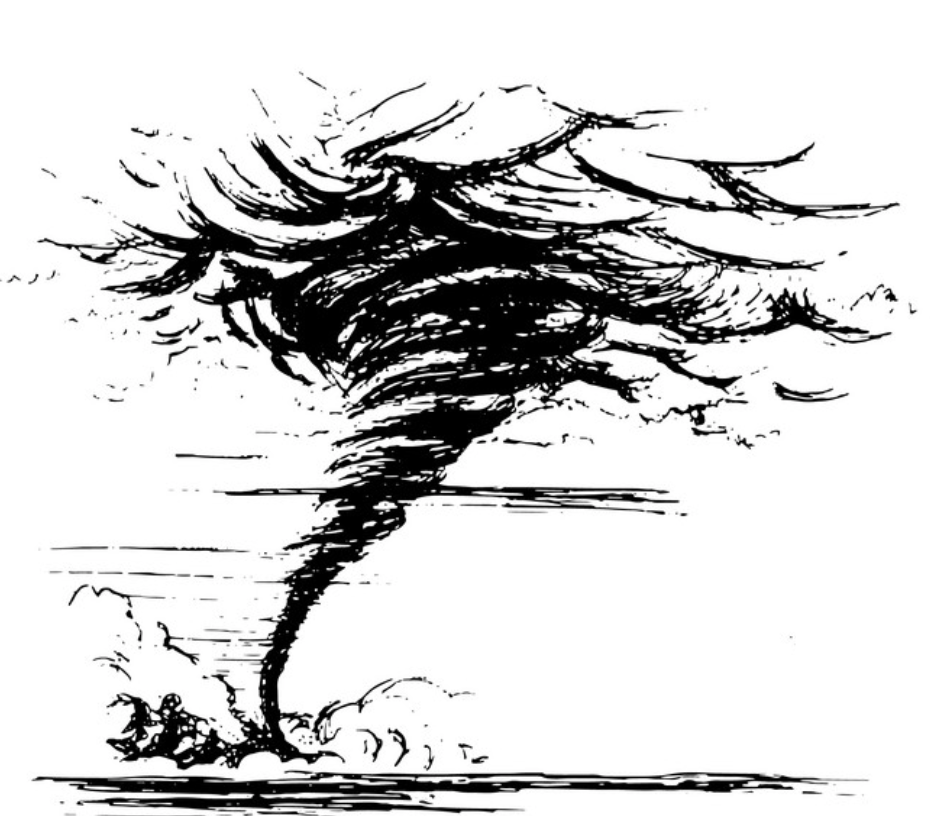
\includegraphics[scale=.6]{resources/tornado}
% \end{center}

{\fontfamily{qpl}\selectfont
\vspace{0.3em}
\begin{mdframed}[style=l3style]
%Synthèse multi-objectif\\dans les processus\\décisionnels de Markov
Multi-objective \\synthesis in Markov \\ Decision Processes
%\vspace{-0.8em} \\\vspace{-0.8em}\HRule % Defines a new command for the horizontal lines, change thickness here
%{\Large Rapport de stage}
\end{mdframed}
}
\umonslogo

\vspace{4em}


\vspace{.3\linewidth}
%\vspace{.1\linewidth}
\begin{adjustbox}{minipage=.6\textwidth,right}
%\Large
\large
\begin{flushright}
\textit{Master thesis submitted by}\\Florent Delgrange\\ \textit{in fulfillment of the requirements for the Computer Science Master degree}\par
\end{flushright}
\textit{Directors : } \par $\quad$ Véronique Bruyère\par
$\quad$ Mickael Randour
\end{adjustbox}
\clearpage % end title page

\newgeometry{a4paper,width=150mm,top=25mm,bottom=35mm}
\let\tmp\oddsidemargin
\let\oddsidemargin\evensidemargin
\let\evensidemargin\tmp
\reversemarginpar

\begingroup
  \pagestyle{empty}
  \null
  \newpage
\endgroup
\tableofcontents
\clearpage % end title page
\begingroup
  \thispagestyle{empty}
  \null
  \newpage
\endgroup
% \include{intro}
% \include{chapter_cc}
% \include{classification1M}
% \include{validation}
% \chapter*{Conclusion}
\addcontentsline{toc}{chapter}{Conclusion}
\markboth{Conclusion}{Conclusion}

\section*{Summary}
\addcontentsline{toc}{section}{Summary}

This thesis presented many decision problems related to the minimisation of costs to reach one or multiple sets of target states in MDPs.
In order to solve these problems, we presented algorithms allowing to build optimal strategies satisfying them.
A summary of the results for each problem is depicted in Table \ref{results-conclusion}.\\

\begin{table}[h]
\centering
\small
\begin{tabular}{|c|c|c|c|c|}
\hline
\textbf{Problem}                                                                                                       & \textbf{Decision time}                           & \multicolumn{3}{c|}{\textbf{Satisfying strategy}} \\ \cline{3-5}
                                                                                                                       &                                                  & \textit{type}   & \textit{memory}   & \textit{optimal}     \\ \hline
\SR{}                                                                                                 & P($\mathcal{M}$)                                 & pure            & memoryless        & yes         \\ \hline
\SSPE{}                                                                                               & P($\mathcal{M}$)                                 & pure            & memoryless        & yes         \\ \hline
\SSPP{}                                                                                               & P($\mathcal{M}$) $\cdot$ P$_{ps}$($\ell$)        & pure            & P$_{ps}$($\ell$)  & yes         \\ \hline
\SPG{}                                                                                                & P($\mathcal{M}$)                                 & pure            & memoryless        & yes         \\ \hline
\SSPWE{}                                                                                              & P($\mathcal{M}$) $\cdot$ P$_{ps}$($\ell$)        & pure            & P$_{ps}$($\ell$)  & yes         \\ \hline
\begin{tabular}[c]{@{}c@{}}\MOSR{}\\ (absorbing target states)\end{tabular}                           & P($\mathcal{M}$)                                 & randomised      & memoryless        & $\epsilon$  \\ \hline
\MOSR{}                                                                                               & P($\mathcal{M}$) $\cdot$ E($\mathcal{Q}$)        & randomised      & E($\mathcal{Q}$)  & $\epsilon$  \\ \hline
\begin{tabular}[c]{@{}c@{}}\SSPPQ{}\\ (unique set of target states\\ + single dimension)\end{tabular} & P($\mathcal{M}$) $\cdot$ P$_{ps}$($\ell_{\max}$) & randomised      & P$_{ps}$($\ell$)  & $\epsilon$  \\ \hline
\SSPPQ{}                                                                                              & P($\mathcal{M}$) $\cdot$ E($\mathcal{Q}$)        & randomised      & E($\mathcal{Q}$)  & $\epsilon$  \\ \hline
\end{tabular}
\caption{Results of problems approached in the thesis. P($x$), E($x$) and P$_{ps}$($x$) respectively denote polynomial, exponential and
 pseudo-polynomial time in parameter $x$. The symbol $\mathcal{M}$ denotes the size of the model, $\ell$ denotes a cost threshold, and $\mathcal{Q}$ denotes the query size. The optimal strategy column describes if it is possible to get an optimal satisfying strategy with the same time complexity that the decision time for a given problem. Moreover, the value $\epsilon$ denotes that it is possible to have an $\epsilon$-approximation of an optimal strategy.}
\label{results-conclusion}
\end{table}


We saw that verifying reachability, persistence, and repeated reachability properties in an MDP requires to solve an \SR{} problem, which consists in deciding the existence of a strategy allowing to reach a set of target states with a probability threshold.
Such a problem can be solved in polynomial time in the size of the model, by linear programming or with an iterative approximation approach called value iteration.
%Optimal pure strategies satisfying such properties can be built in polynomial time in the size of the model and do not require memory, except for the constrained bounded-step reachability, in which case the size of the memory is linear in the number of bounded steps required
\\

By considering cost of paths, we first assumed actions of MDPs having a single-dimension weight, and we saw that the \SSPE{} problem, consisting in deciding the existence of a strategy ensuring good expected cost-to-target, can be decided in polynomial time in the size of the model, by linear programming or with the value iteration approach.
% Optimal pure strategies satisfying such a property can be built in polynomial time and do not require memory.
%Then, we have seen that deciding the existence of a strategy ensuring a
Then, we saw that verifying a cost-bounded property in any MDP
%can be decided in pseudo-polynomial time in the size of the model and in the length of the cost threshold.
requires to solve an \SSPP{} problem, consisting in deciding the existence of a strategy allowing to reach a set of target states with a cost bounded and with a probability threshold.
The resolution of this problem requires to build an unfolding of the model up to the cost threshold, leading a pseudo-polynomial time in the size of the model and in the length of this cost threshold.\\
% Optimal pure strategies satisfying such properties can therefore be computed in pseudo-polynomial time and additionally requires pseudo-polynomial memory. \\

Afterwards, we presented the \SPG{} problem, consisting in deciding the existence of a strategy allowing to guarantee a worst case threshold (in terms of cost) to reach a set of target states.
Inspired by a turn-based two-player game approach, we saw that this problem
can be solved by dynamic programming, without unfolding the model.
%can be decided in polynomial time in the size of the model by dynamic programming and optimal memoryless pure strategies satisfying this problem can be built in polynomial time in the size of the model and do not require memory.
This allowed us to present the multi-objective \SSPWE{} problem, consisting in deciding the existence of a strategy offering a worst case guarantee of reaching a set of target states while ensuring a good expectation to reach this set of target states.
A solution to this problem was approached by unfolding the MDP up to the worst case threshold, and limiting its state space to the attractor of the set of target states for which cost of paths has not exceeded the worst case threshold.\\
% Therefore, the problem can be decided in pseudo-polynomial time in the size of the model and in the length of the worst case cost threshold.
% Optimal pure strategies satisfying it can be built in pseudo-polynomial time and require pseudo-polynomial memory.\\

Then, we presented the \MOSR{} problem, consisting in deciding the existence of a strategy satisfying multiple reachability to multiple set of target states, with multiple probability thresholds.
Such a problem induces compromises between satisfying strategies, and we defined the notion of Pareto curve, allowing to deal with these compromises.
Indeed, according to a given multi-objective problem, each point of this Pareto curve is actually linked to a (Pareto-)optimal strategy satisfying the problem.
We saw that in the case where all target states are absorbing, the problem can be decided in polynomial time in the size of the model by linear programming.
% and a randomised strategy satisfying the problem can be built in polynomial time and does not require memory.
Furthermore, building Pareto-optimal strategies for the problem can be done by enumerating vertices of the Pareto curve, that can be $\epsilon$-approximated in polynomial time in the model and in $\frac{1}{\epsilon}$.
Based on these results, we approached the general case, where all the targets states are not necessarily absorbing, by exponentially increasing the size of the state space of the MDP, according to the number of reachability properties to satisfy, and by considering the maximal end components of this modified MDP.
%It followed that the problem can be decided in polynomial time in the size of the model, but exponential time in the number of reachability properties.
%A randomised satisfying strategy can thus be built in exponential time and requires exponential memory, while
In that case, an $\epsilon$-approximation of the Pareto curve can be built in polynomial time in the size of the model and $\frac{1}{\epsilon}$, but in exponential time in the number of reachability properties.\\

For the last problem, we have considered multi-dimensional MDPs, where actions have multiple weights.
We approached the \SSPPQ{} problem, consisting in deciding the existence of a strategy allowing to satisfy multiple percentile queries.
Each of these queries consists in reaching a set of target states with a cost bounded on a given dimension and with a probability threshold.
We approached the problem by unfolding the MDP up to the highest cost threshold, on all its dimensions, necessarily leading to an exponential time decision, and by solving then an \MOSR{} problem for the target states in this unfolding.
The results for absorbing target states in the \MOSR{} problem allowed to improve this exponential time to a pseudo-polynomial time in the size of the model and in the length of the highest cost threshold for simultaneously single-dimension and single-target queries.\\

Finally, we introduced a modern model checker called Storm, allowing to model-check Markov decision processes, and supporting all the problems presented in this thesis.
We presented some input languages allowing to encode MDPs in Storm, and the probabilistic branching time logic of Storm, allowing to express properties to verify and query a given MDP.

\subsection*{Future work}
\addcontentsline{toc}{section}{Future work}
  \subsubsection*{Other cost measures}
    In this thesis, we have considered cost of paths in MDPs with the truncated sum function (i.e., $\TS$), that is perfectly suited for variations of the shortest path problem in MDPs.
    There actually are many other measures:
    \begin{itemize}
      \item the \textit{discounted sum}, modelling that short-term costs are more important than long-term ones \cite{DBLP:journals/fmsd/RandourRS17},
      \item the \textit{mean-payoff}, describing the long-run average cost per executed action in a path \cite{DBLP:journals/corr/BruyereFRR13},
      \item etc.
    \end{itemize}
    It should be interesting to consider them and study multi-objective problems related to these measures.
  \subsubsection*{\textbf{Game-based abstraction}}
  It is possible to reduce the size of MDPs by stochastic two-player game-based abstraction for a given reachability, or expected cost-to-target problem \cite{DBLP:journals/fmsd/KattenbeltKNP10}.
  It could be useful to consider such abstraction techniques for multi-objective problems.

  \subsubsection*{\textbf{Reinforcement learning for strategies}}
     Multiple machine learning techniques have been presented in  \cite{10.1007/978-3-319-11936-6_8} to improve performance by avoiding an exhaustive exploration of the state space, yielding precise lower and upper bounds to verify required properties.
    Again, it could be interesting to investigate the use of related techniques to verify multi-objective properties in Markov decision processes.

  \subsubsection*{\textbf{Reward-epoch model}}
    In order to optimise the time
    complexity for the multi-objective problems requiring
    an unfolding, a way to avoid this unfolding have been introduced in \cite{10.1007/978-3-319-89963-3_19} by only looking at interesting states of the unfolding (intuitively, the model is implicitly unfolded along reward epochs, and the regularities of a modification of the MDP, called epoch-model of the MDP, are exploited).
    It is actually the method used in Storm to verify multi-objective cost-bounded properties in a given MDP.

  \subsubsection*{\textbf{Storm}}
    Moreover, as Storm is open-source, we can enrich this model checker with
    new algorithms.
    Indeed, for instance, the exploration and abstraction engines (cf. Section \ref{engines}) do not support yet\footnote{ in the version of Storm 1.2.0} the multi-objective problems.


\chapter{State of the art}
\textit{This chapter refers to (and summarizes) my Master project. Concepts and definitions are essentially inspired by the chapter ten of the book ``Principles of model checking'' \cite{PMC}, the chapter ``Model checking probabilistic systems'' of the Mickael Randour course named ``Formal verification of computer systems'' \cite{MRV} as well as the article ``Variations on the stochastic shortest path problem'' \cite{DBLP:journals/corr/RandourRS14a}.} \\

Before studying different multi-objective problems in \textit{Markov decision
processes} and defining \textit{strategies} that solve such problems, we will introduce some fundamental concepts that define the area of the subject.
Actually, we will be interested to know some measurements related to the cost of \textit{paths} of Markov decision processes as well as to the probability to reach some states in these models through these paths.
These measurements can not be computed without defining a probability measure on events formed with these paths.
So, first of all, we need to define what are \textit{Markov chains}. Indeed, these
stochastic models are essential to measure the probability of \textit{paths} of Markov decision processes.

\section{Markov chains}
Markov chains are transitions system based models that describe the evolution of situations in stochastic environments.
%The particularity of such systems is that each state inside these models can go to its successors following a probability distribution.
The particularity of a such system is that it can evolve from any state to one of its successors following a probability distribution.
%That yields that a Markov chain being in a state and evolving to another one only depends on this state.
That yields that the evolution of a Markov Chain, i.e., to go from a state to another one, only depends on the current state of the system.
\begin{definition}[\textbf{Discrete-time Markov chain}]
  A \textit{(weighted) discrete-time Markov chain} (denoted by \textbf{MC}) is a stochastic model defined by a tuple $\mathcal{M}=(S, \Delta, w, AP, L)$ where
	\begin{itemize}
		\item $S$ is a countable set of states,
		\item $\Delta: S \times S \rightarrow [0,1] \cap \mathbb{Q}$ is a  \textit{transition function} such that \[\forall s \in S, \sum_{s' \in S}\Delta(s, s')= 1\]
		%\item $d_0:S \rightarrow [0,1]$ est la distribution initiale telle que \[\sum_{s \in S}d_0(s)= 1\] (à noter que dans le cadre de ce document, la distribution initiale peut être omise, et dans ce cas, $\forall s \in S, d_0(s) = \frac{1}{|S|}$).
		where $\Delta(s, s')$ describes the probability that the system goes from state $s$ to state $s'$ in one transition,
    \item $w: S \times S \rightarrow \mathbb{N}_0$ %est la fonction
        %de poids associant à chaque transition un coût strictement positif.
      is a weight function that links a strictly positive cost to each transition,
    \item $AP$ is a set of atomic propositions, and
    \item $L: S \rightarrow 2^{AP}$ is a labeling function.
	\end{itemize}
  \textit{Remark }: $AP$ and $L$ can be ommited. In that case, we consider that $AP = S$ and $L$ is the natural labeling of each state, i.e., for all $s \in S$, $L(s) = \{s\}$
\end{definition}

\begin{property}
  Let $\mathcal{M} = (S, \Delta, w, AP, L)$ be an MC and $s \in S$ be a state of $\mathcal{M}$. The transition function $\Delta$ defines a probability distribution $\Delta_s: S \rightarrow \mathcal{D}(S), \, s' \mapsto \Delta(s, s')$ on $S$.
\end{property}

We can represent an MC $\mathcal{M} = (S, \Delta, w, AP, L)$ with a directed graph, where vertices represent states
of the MC and where any edge $(s, s') \in S^2$, that links two states, is labeled with the nonzero transition probability to go from $s$ to $s'$, i.e., $\Delta(s, s')$, as well as the cost of this transition, i.e., $w(s, s')$.
We name this graph the \textit{underlying graph of} $\mathcal{M}$.
Additionally, labels of each
state can be represented next to it.

\begin{notation}[\textit{Size of an MC}]
  An MC $\mathcal{M}=(S, \Delta, w, AP, L)$ is called \textit{finite} if its state space $S$ is finite. The size of $\mathcal{M}$ corresponds to the size of the set
  $\{(s, s') \in S^2 \; | \; \Delta(s, s') > 0 \}$, i.e., the number of edges in the underlying graph of $\mathcal{M}$.
\end{notation}

\begin{example}[\textit{Production of solar panels according to weather}]\label{solar-panel}
  Let $\mathcal{M}_{sp} = (S, \Delta, w, AP, L)$ be the MC of the figure \ref{MCexample}. This system modelises the production of energy (in $kJ$) of
  an installation of solar panels, according to weather.
  Here, the states are elements of $S = \{s_0, s_1, s_2, s_3\}$ and the atomic propositions are elements of $AP = \{sunny, \, slightly\_cloudy, \, moderately\_cloudy, \, cloudy \}$. The transition function is given by edges on the figure (e.g., $\Delta(s_0, s_1) = \frac{1}{5}$) as well as the
  cost of each transition (e.g., $w(s_0, s_1) = 5$). finally, labels of states
  are put next each of them in orange in the figure (e.g., $L(s_0) = \{sunny\}$).
  \begin{figure}[h!]
    \centering
    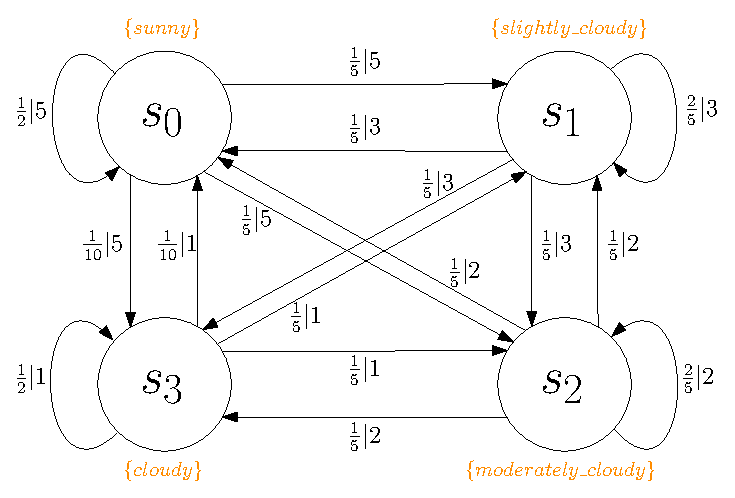
\includegraphics[width=0.6\linewidth]{resources/weather-solar-pannel}
    \caption{MC modeling a daily production of energy (in $kJ$) of solar panels according to weather}
    \label{MCexample}
  \end{figure}
  The way $w$ is defined for this MC yields that, when a day is sunny, the installation produces $5 kJ$ during this day, $3 kJ$ when a day is slightly cloudy, $2 kJ$ when a day is moderately cloudy and, finally, $1 kJ$ when the day is cloudy.
\end{example}

\subsection{Paths of Markov chains}
Before addressing how to compute probabilities in MCs, we must introduce the notion of paths in MCs. Actually, probabilistic events of MCs are sets of paths and prefixes of paths are used to generate these events.
\begin{definition}[\textbf{Paths of an MC}] Let $\mathcal{M} = (S, \Delta, w, AP, L)$ be an MC.
A \textit{path} $\pi = s_0 s_1 s_2 \dots$ of $\mathcal{M}$ is a (infinite) sequence of states of the MC such that for all $i \in \mathbb{N}$, $\Delta(s_i, s_{i+1})> 0$. We denote by $Paths(s)$ the set of paths $\pi = s_0s_1s_2\dots$ of $\mathcal{M}$ starting from the state $s \in S$, i.e., such that $s_0 = s$.
\end{definition}
\begin{definition}[\textbf{Finite paths of an MC}]
Let $\mathcal{M} = (S, \Delta, w, AP, L)$ be an MC.
A \textbf{finite} path $\hat{\pi} = s_0 \dots s_n$ of $\mathcal{M}$, with $n \in \mathbb{N}$, is a finite sequence of states of $\mathcal{M}$ such that $\Delta(s_i, s_{i+1}) > 0$ for all $i \in \{0, \dots, n-1\}$.
We denote by $Paths_{fin}(s)$ the set of finite paths $\hat{\pi} = s_0 \dots s_n$ starting from the state $s \in S$, i.e., such that $s_0 = s$
\end{definition}
\begin{definition}[\textbf{Prefixes of paths}]
Let $\mathcal{M} = (S, \Delta, w, AP, L)$ be an MC and $\pi = s_0s_1s_2 \dots$ be a path of $\mathcal{M}$. A prefix of $\pi$ is a finite path $\hat{\pi} = s'_0 \dots s'_n$, with $n \in \mathbb{N}$, such that $s'_i = s_i$ for all $i \in \{0, \dots, n\}$.
The set of all prefixes of $\pi$ is denoted by $pref(\pi)$.
\end{definition}

\subsection{Probabilities and events in Markov chains}

We are now interested in probabilistic events of MCs and how measuring them. These events can be formulated with the notion of \textit{cylinder set}.

\begin{definition}[\textbf{Cylinder set}]
Let $\mathcal{M} = (S, \Delta, w, AP, L)$ be an MC, $s \in S$ be a state of $\mathcal{M}$ and $\hat{\pi} \in Paths_{fin}(s)$ be a finite path of $\mathcal{M}$.
\[Cyl(\hat{\pi})=\{\pi\in Paths(s)\;|\;\hat{\pi}\in pref(\pi) \} \]
\end{definition}

We can express all events with this formulation. For example, the event that consists of a singleton containing just a single path $\pi = s_0s_1\dots$ is given by $\bigcap_{\hat{\pi} \in pref(\pi)} Cyl(\hat{\pi})$

\begin{theorem}\label{theo1}
  Let $\mathcal{M}=(S, \Delta, w, AP, L)$ be an MC and $s \in S$ be a state of $\mathcal{M}$. There exists a unique probability measure $\mathbb{P}_s$ on the
  $\sigma$-algebra over $Paths(s)$ where the probabilities of cylinder sets (i.e., of events) are given by
  \[
    \mathbb{P}_s(Cyl(s_0 \dots s_n)) = \prod_{i = 0}^{n - 1} \Delta(s_i, s_{i+1})
  \]
  whit $s_0 = s$ and $n \in \mathbb{N}$.
\end{theorem}
\begin{corollary}
Any event defined using complementation or countable union of cylinder sets are also measurable.
\end{corollary}

\begin{example}[\textit{Measuring an event of an MC modeling a solar panel system}]
  Let $\mathcal{M}_{sp} = (S, \Delta, w, AP, L)$ be the MC of the example \ref{solar-panel}. The probability of sunny weather four days in a row starting on a sunny day is given
  by $\mathbb{P}_{s_0}(Cyl(s_0s_0s_0s_0)) = (\frac{1}{2})^3 = \frac{1}{8}$
\end{example}

\subsection{Objectives in Markov chains}

With this background, we can now introduce some classical problems that consist
of completing an objective in an MC. The first one that we will tackle is the reachability problem.
%\subsubsection{Reachability problem}
\begin{definition}[\textbf{Reachability event}]
  Let $\mathcal{M} = (S, \Delta, w, AP, L)$ be an MC and $T \subseteq S$ be a set of target states. The event of reaching $T$, denoted by $\Diamond T$,
  is defined as a finite union of cylinder sets. Indeed, let $s \in S$ be a state of $\mathcal{M}$ and $Paths_{fin}^T(s)$ be the set of finite paths $\hat{\pi} = s_0 \dots s_n \in Paths_{fin}(s)$, such that for all $i \in \{0, \dots, n-1 \}, \, s_i \not \in T$ and $s_n \in T$,
  \[ \Diamond T = \bigcup_{s_0 \dots s_n \in Paths_{fin}^T(s)} Cyl(s_0 \dots s_n) \]
  Since all cylinders of the set $Paths_{fin}^T(s)$ are disjoint (their prefixes are different), we can measure $\Diamond T$ with:
  \[
    \mathbb{P}_s(\Diamond T) = \sum_{s_0 \dots s_n \in Paths_{fin}^T(s)}  \mathbb{P}_s(Cyl(s_0 \dots s_n))
  \]
\end{definition}
It remains to compute this probability.

\begin{theorem}
Computing $\mathbb{P}_s(\Diamond T)$ for all $s \in S$ can be done in polynomial
time through a linear equations system (cf. appendix \ref{app-reach} for more details).
\end{theorem}

% \begin{example}[\textit{Reachability property in an MC modeling a solar panel system}]
%   Let $\mathcal{M}_{sp}$ be the MC modeling the system of the example \ref{solar-panel}.
%    The probability that a cloudy day eventually comes, starting on a sunndy day, is one, i.e., $\mathbb{P}_{s_0}(\Diamond \{s_3\}) = 1$. Indeed, the underlying graph of $\mathcal{M}_{sp}$ is strongly connected, so reaching any state starting from any state has always a probability $1$.
% \end{example}

Now, we will consider the \textit{cost of paths} of an MC. Furthermore, we
are interrested by the cost of paths to reach $T$. To compute this cost, we use the \textit{truncated sum function}.

\begin{definition}[\textbf{Truncated sum}]
  Let $\mathcal{M}=(S, \Delta, w, AP, L)$ be an MC, $s \in S$ be a state of $\mathcal{M}$, $\pi = s_0s_1s_2\dots \in Paths(s)$ be a path of $\mathcal{M}$ and $T \subseteq S$ be a set of target states.
  The trunacted sum of $\pi$ is the cost to reach $T$ through $\pi$
  for the first time. More formally, the function $TS^T: Paths(s) \rightarrow \mathbb{N} \cup \{\infty\}$ is defined as follows:
	\[
		TS^T(\pi) =
		\begin{cases}
			\sum_{i = 0}^{n-1} w(s_i, s_{i+1}) & \quad \text{if } \forall i \in \{0, \dots, n - 1\}, s_i \not\in T \text{ and } s_n \in T \\
			\infty & \quad \text{else, if } \forall i \in \mathbb{N}, \, s_i \notin T
		\end{cases}
	\]
\end{definition}
With this function, it is now possible to introduce the concept of
expected cost of paths of an MC to reach a set of targets as well as
the probability of reaching this target set with a cost bounded.

\begin{definition}[\textbf{Expected cost of paths of an MC for reachablity properties}]
	Let $\mathcal{M} = (S, \Delta, w, AP, L)$ be an MC, $s \in S$ be a state of $\mathcal{M}$ and $T \subseteq S$ be a set of target states. We define the expected cost to reach $T$, i.e., $\mathbb{E}_s(\Diamond T)$, corresponding to \textit{the expected truncated sum of paths from $s$ to reach $T$} as follows:
	\begin{itemize}
	\renewcommand{\labelitemi}{\tiny$\bullet$}
	\item If $\mathbb{P}_s(\Diamond T) < 1$, then $\mathbb{E}_s(\Diamond T) = \infty$.%(par la propriété \ref{prop-ts}).
	\item Else, if $\mathbb{P}_s(\Diamond T) = 1$, then:
	\[
    \mathbb{E}_s(\Diamond T) = \sum_{c = 0}^\infty c \cdot \mathbb{P}_s(\{\pi \in Paths(s) \; | \; TS^T(\pi) = c \})
  \]
	\end{itemize}
\end{definition}

An equivalent characterisation of the expected cost from $s \in S$ to $T$ in case of $\mathbb{P}_s(\Diamond T) = 1$ is given by
\[
  \mathbb{E}_s(\Diamond T) = \sum_{\hat{\pi} \in Paths_{fin}^T(s)} \mathbb{P}_s(Cyl(\hat{\pi})) \cdot TS^T(\hat{\pi})
\]
with $Paths^T_{fin}(s)$, the set of finite paths $\hat{\pi} = s_0 \dots s_n \in Paths_{fin}(s)$  such that, for all $i \in \{0, \dots, n-1\}, s_i \not \in T$ and $s_n \in T$. Since we can measure the probability of cylinder sets of finite paths of $\hat{\pi} \in Paths_{fin}^T(s)$, we can compute $\mathbb{E}_s(\Diamond T)$.

\begin{theorem}
  Computing $\mathbb{E}_s(\Diamond T)$ for all $s \in S$ can be done in polynomial time through a linear equations system (cf. appendix \ref{app-expMC} for more details).
\end{theorem}

The last concept that we will define in MCs is the cost bounded reachability.

\begin{definition}[\textbf{Cost bounded reachability probability}]
	Let $\mathcal{M} = (S, \Delta, w, AP, L)$ be an MC, $s \in S$ be a state of $\mathcal{M}$, $T \subseteq S$ be a set of target states and $l \in \mathbb{N}$ be a length threshold.
  The \textit{probability to reach $T$ from $s$ with a cost bounded} by the threshold $l$ is defined as follows:
	\[
    \mathbb{P}_s(\Diamond_{\leq l} T) = \mathbb{P}_s(\{\pi \in Paths(s) \; | \; TS^T(\pi) \leq l \})
  \]
\end{definition}
The event $\{\pi \in Paths(s) \; | \; TS^T(\pi) \leq l \}$ is actually measurable
in the unfolded MC until $l$.
\begin{theorem}
  The probability of the cost bounded reachability to a set of target states $T \subseteq S$ from a state $s \in S$ can be computed in pseudo-polynomial time in the size of $\mathcal{M}$ and $l$, through an unfolding of $\mathcal{M}$ until $l$.
\end{theorem}

Intuitively, we unfold $\mathcal{M}$ by recording in each state the cost of
current paths. The new set of target states in the unfolded MC is the set of
target states in $\mathcal{M}$ that have a current cost less than $l$ (cf.
appendix \ref{app-cbrMC} for more details). Finally, it remains to compute the probability to
reach these new target states in the unfolded MC. \\

Now, we can define what is a Markov decision process and introduce the concept of strategy, that is the pillar concept of resolving objective problems in such models.

\section{Markov decision processes}
Markov decision processes are systems that modelise situations describing both non-deterministic and stochastic evolution. Indeed, in comparison with Markov chains, a Markov decision process requires a decision making to go from a state of the model to its successors. After that, the system evolves following the probability distribution formed by this state and the decision taken.

\begin{definition}[\textbf{Markov decision process}]
	A \textit{Markov decision process}, (denoted by \textbf{MDP}) is defined by a tuple $\mathcal{M}  = (S, A, \Delta, w, AP, L)$ where
	\begin{itemize}
		\item $S$ is a countable set of states,
		\item $A$ is a countable set of actions ; we denote by $A(s) \in 2^A$  the set of enabled actions when the system is in state $s$ such that, for all $s \in S$,
    $A(s) \neq \emptyset$,
		\item $\Delta: S \times A \times S \rightarrow [0, 1] \cap \mathbb{Q}$ is the probability transition function such that
		\begin{flalign*}
			&\forall s \in S, \; \forall \alpha \in A(s), \; \sum_{s' \in S} \Delta(s, \alpha, s') = 1 \\
			\text{and } &\forall s, s' \in S, \; \forall \alpha \in A \setminus A(s), \; \Delta(s, \alpha, s') = 0
		\end{flalign*}

			where $\Delta(s, \alpha, s')$ defines the probability of going from $s$ to $s'$ in one transition when the action $\alpha \in A(s)$ is chosen,
    \item $w: A \rightarrow \mathbb{N}_0$ %est la fonction
        %de poids associant à chaque transition un coût strictement positif.
      is a weight function that links a strictly positive cost to each action,
    \item $AP$ is a set of atomic propositions, and
    \item $L: S \rightarrow 2^{AP}$ is a labeling function.
	\end{itemize}
  \textit{Remark: }again, $AP$ and $L$ can be ommited. In that case, we consider that $AP=S$ and $L$ is the natural labeling of each state, i.e., for all state $s \in S$, $L(s) = \{s\}$.
\end{definition}

\begin{property}
  Let $\mathcal{M} = (S,A, \Delta, w, AP, L)$ be an MDP, $s \in S$ be a state of $\mathcal{M}$ and $\alpha \in A(s)$ be an enabled action of the state $s$. The transition function $\Delta$ defines a probability distribution $\Delta_{s, \alpha}: S \rightarrow \mathcal{D}(S), \, s' \mapsto \Delta(s, \alpha, s')$ on $S$.
\end{property}
\begin{property}
  An MC is essentially an MDP where, for each state $s$, $|A(s)| = 1$.
\end{property}

We will now introduce some useful notations.

\begin{notation}
  Let $\mathcal{M}=(S, A, \Delta, w, AP, L)$ be an MDP,
  \begin{itemize}
    \item $Pred(s) = \{ s' \in S \; | \; \exists \alpha \in A(s'), \, \Delta(s', \alpha, s) > 0 \}$ is the set of predecessors of the state $s \in S$ in the the MDP,
    \item $Succ(s) = \{ s' \in S \; | \; \exists \alpha \in A(s), \, \Delta(s, \alpha, s') > 0 \}$ is the set of successors of the state $s \in S$ in the MDP and
    \item $Succ(s, \alpha) = \{ s' \in S \; | \; \Delta(s, \alpha, s') > 0 \}$
      is the set of $\alpha$-successors of the state $s \in S$ in the MDP, i.e., the set of possible successors of $s$ when the action $\alpha$ is chosen
  \end{itemize}
\end{notation}

%The underlying graph of an MDP $\mathcal{M}$ is a directed graph where vertices are states of $\mathcal{M}$ and each edge starting from a state $s$ to one of its successor $s'$ exists if and only if there exists an enabled action $\alpha$
%of $s$ such that $\Delta(s, \alpha, s') > 0$. For the other elements of the tuple defining $\mathcal{M}$, the graph is essentially caracterised the same way as for an MC.
We can represent an MDP with its underlying directed graph, the same way as for an MC, with the exception that each vertex representing a state $s$ has outgoing edges to intermediate vertices representing enabled actions of $s$ and, for each enabled action $\alpha$ of $s$, edges go from the vertex representing $\alpha$ to vertices representing $\alpha$-successors of $s$.

\begin{notation}[\textit{Size of an MDP}]
  An MDP $\mathcal{M}=(S, A, \Delta, w, AP, L)$ is called \textit{finite} if its state space $S$ is finite. The size of $\mathcal{M}$ corresponds to the size
  of the set $\{(s, \alpha, s') \in S \times A \times S \; | \; \Delta(s, \alpha, s') > 0 \}$, i.e., the number of outgoing edges of vertices representing actions in the underlying graph of $\mathcal{M}$.
\end{notation}

\begin{example}\label{simple-mdp}
  Let $\mathcal{M} = (S, A, \Delta, w, AP, L)$ be the MDP of the figure \ref{mdp01}. We have that $S = \{s_0, s_1, s_2\}$, $A = \{\alpha, \beta, \gamma\}$ and $AP=\{a, b\}$. If the system currently is in state $s_0$, labeled with $L(s_0) = \{a\}$, the only action available is $\beta$ (because $A(s_0) = \{\beta\}$).
  The cost of choosing $\beta$ is $w(\beta) = 3$.
  Thus, the system evolves following the probability distribution defined by $\Delta_{s_0, \beta}$: it has a probability of $\frac{1}{2}$
  to go to its $\beta$-successor $s_1$ and a same probability to go to its $\beta$-successor $s_2$. Let assume that the system evolves to the state $s_2$, a state with no label ($L(s_2) = \emptyset$). So, in that case, the system has two possible decisions: $\alpha$ or $\gamma$ (because $A(s_2) = \{\alpha, \gamma\}$). If $\alpha$ is chosen, the system returns to $s_2$ with a probability one and a cost of $w(\alpha) = 5$. Else, if $\gamma$ is chosen, the system goes to $s_0$ with a probability one and a cost of $w(\gamma) = 2$.
  \begin{figure}[h!]
    \centering
    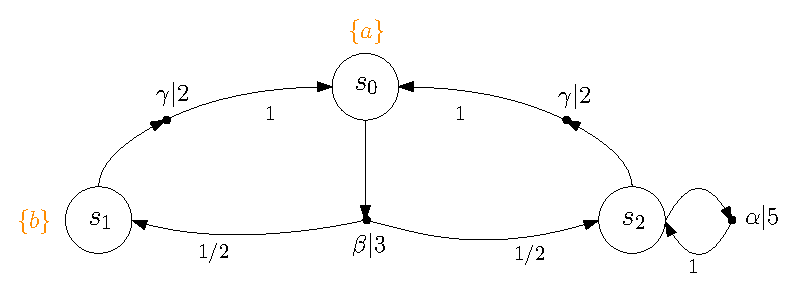
\includegraphics[width=0.7\linewidth]{resources/simple-mdp}
    \caption{MDP with $3$ states, $3$ actions and $2$ atomic propositions}\label{mdp01}
  \end{figure}
\end{example}

\subsection{Strategies in Markov decision processes}
In order to resolve nondeterminism inside MDPs, we need the notions of paths in MDPs and strategies.
\begin{definition}[\textbf{Paths in an MDP}]
  Let $\mathcal{M}=(S, A, \Delta, w, AP, L)$ be an MDP and the transition relation
  \[\rightarrow \; =  \{ (s, \alpha, s') \in S \times A \times S \; | \; \Delta(s, \alpha, s') > 0 \}, \,\]
	a path $\pi$ of $\mathcal{M}$ is defined as a sequence of states and actions
	\[ \pi = s_0 \xrightarrow{\alpha_1} s_1 \xrightarrow{\alpha_2} s_2 \xrightarrow{\alpha_3} \dots \]
	Let $s \in S$ be a state of $\mathcal{M}$, we denote by $Paths(s)$ the set of
	paths of $\mathcal{M}$ starting from the state $s$, i.e., such that $s_0 = s$.
\end{definition}
In opposition of MCs, there is no probabilistic space defined on paths of MDPs.
This is related to nondeterminism linked to the choices of possible actions when the system is in a state. We need strategies to resolve nondeterminism.
\begin{definition}[\textbf{Histories}]
	Let $\mathcal{M} = (S, A, \Delta, w, AP, L)$ be an MDP. An \textit{history} of $\mathcal{M}$
	is a finite sequence of states $(s_0 \dots s_n) \in S^+$ where, for all
	$i \in \{1, \dots, n \}, \; \exists \alpha \in A(s_{i-1})$ such that $\Delta(s_{i-1}, \alpha, s_i) > 0$.
	An history is the sequence of states that brought the state $s_0$ to the state $s_n$ along a path of $\mathcal{M}$. The set of histories of $\mathcal{M}$  is given by $\mathcal{H}(S)$.
\end{definition}

These notions allow to introduce strategies in MDPs.

\begin{definition}[\textbf{Pure strategy}]
Let $\mathcal{M} = (S, A, \Delta, w, AP, L)$ be an MDP. A \textit{strategy} (also named \textit{policy} or \textit{scheduler} in literature) for $\mathcal{M}$
	is a function
	$\sigma: \mathcal{H}(S) \rightarrow A$
	that selects, for a given history $h = (s_0 \dots s_n) \in \mathcal{H}(S)$, an enabled action of $s_n$, i.e., $\sigma(s_0 \dots s_n) = \alpha \in A(s_n)$.
	The path $\pi = s_0 \xrightarrow{\alpha_1} s_1 \xrightarrow{\alpha_2} s_2 \xrightarrow{\alpha_3} \dots$
	is a $\sigma$-path iff $\alpha_i = \sigma(s_0 \dots s_{i-1})$
	for all $i \in \mathbb{N}_0$. The set of $\sigma$-paths starting from the state $s \in S$ is given by $Paths^\sigma(s)$.
\end{definition}
Strategies that we study here are \textit{pure}, i.e., each action is chosen by strategy with probability one. We will see later that \textit{randomised} strategies exist and are essential to resolve some types of problems in MDP. \\

If a strategy controls the decisions of an MDP, then the nondeterminism is solved
and the MDP acts like an MC. Actually, an MDP $\mathcal{M}$ controlled by a strategy $\sigma$ can be formalised as an MC $\mathcal{M}^\sigma$.

\begin{definition}[\textbf{Markov chain induced by strategy}]
Let $\mathcal{M} = (S, A, \Delta, w, AP, L)$ be an MDP and $\sigma$ be a strategy for
$\mathcal{M}$. The MC induced by $\sigma$ is given by
$ \mathcal{M}^\sigma = (\mathcal{H}(S), \Delta^\sigma, w^\sigma, AP, L^\sigma) $, where, for all history
$h = s_0 s_1 \dots s_n$ of $\mathcal{M}$,
\begin{itemize}
\item $\Delta^\sigma(h, h . s_{n+1}) = \Delta(s_n, \sigma(h), s_{n+1})$
\item $w^\sigma(h, h . s_{n+1}) = w(\sigma(h))$
\item $L^\sigma(h . s_{n+1}) = L(s_{n+1})$
\end{itemize}
\end{definition}

\begin{property}
  Let $\mathcal{M}$ be an MDP, $\sigma$ be a strategy on $\mathcal{M}$ and $s\in S$ be a state of $\mathcal{M}$. There exists a bijection between the
  set $Paths^\sigma(s)$ on $\mathcal{M}$ and the set $Paths(s)$ on the MC induced by the strategy $\sigma$, $\mathcal{M}^\sigma$.
\end{property}

Since events of an MC is measurable, events of an MDP controlled by strategy is also measurable.
\begin{notation}
  We denote by $\mathbb{P}_s^\sigma$ the probability measure defined on paths starting from the state $s$ of the Markov chain induced by the strategy $\sigma$.
\end{notation}

Markov chains induced by such (infinite memory) strategies can be seen as forests of trees representing an infinite unfolding of the MDP where actions are controlled by strategy (this is due to the fact that the set of histories of an MDP is infinite). So, such induced MCs have infinite size. Actually, such strategies are not easy to use in practice because it requires to
know the complete history of the system to decide which action to choose. \textit{Finite memory strategies} allow to avoid this problem.

\begin{definition}[\textbf{Finite memory strategy}]
Let $\mathcal{M} = (S, A, \Delta, AP, L)$ be an MDP.
A \textit{finite memory strategy} $\sigma = (Q, \sigma_\alpha, \delta, \delta_0)$ is a \textit{Moore machine} where
\begin{itemize}
	\item $Q$ is a finite set of \textit{modes},
	\item $\sigma_\alpha: Q \times S \rightarrow A$ is a function that chooses, for any $s \in S$, an action $\alpha \in A(s)$ following a mode $q \in Q$ in which the machine currently is,
	\item $\delta: Q \times S \rightarrow Q$ is the transition function,
	\item $\delta_0: S \rightarrow Q$ is the function that chooses the initial mode of the machine following a state $s \in S$ of the MDP from which the machine is initialised.
\end{itemize}
\end{definition}

\begin{definition}[\textbf{Product of an MDP by a strategy}]
Let $\mathcal{M} = (S, A, \Delta, w, AP, L)$ be an MDP and $\sigma = (Q, \sigma_\alpha, \delta, \delta_0)$ be a finite memory strategy for $\mathcal{M}$.
The product of $\mathcal{M}$ by $\sigma$ is given by
\[ \mathcal{M} \times \sigma = \mathcal{M}^\sigma = (S \times Q, \Delta^\sigma, w^\sigma, AP, L^\sigma) \]
where $\mathcal{M}^\sigma$ is the MC induced by the finite memory strategy $\sigma$ and where,
for all states $s, s' \in S$ and for all modes $q, q' \in Q$ of the strategy,
\begin{itemize}
	\item $\Delta^\sigma((s, q), (s', q')) =
	\begin{cases}
	\Delta(s, \sigma_\alpha(q, s), s') & \text{if } \delta(q, s) = q'\\
	0  & \text{else}
	\end{cases}$
  \item $w^\sigma((s, q), (s', q')) = w(\sigma_\alpha(q, s))$
  \item $L^\sigma(s, q) = L(s)$
\end{itemize}
\end{definition}

\begin{example}[\textit{Product of an MDP by a strategy}]
  Let $\mathcal{M}=(S, A, \Delta, w, AP, L)$ be the MDP of the example \ref{simple-mdp} and $\sigma = (Q, \sigma_\alpha, \delta, \delta_0)$ be the
  finite memory strategy of the figure \ref{finite_mem_strat}.
  \begin{figure}[h!]
    \centering
    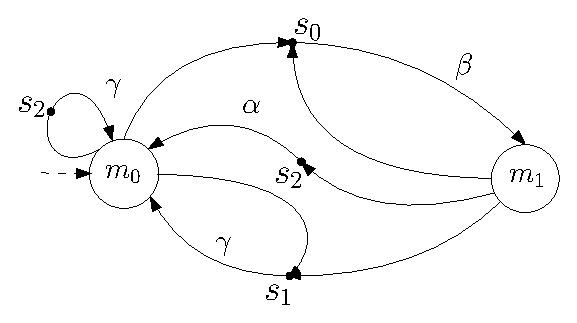
\includegraphics[width=0.4\linewidth]{resources/strategy}
    \caption{Finite memory strategy for $\mathcal{M}$ with $2$ modes}\label{finite_mem_strat}
  \end{figure}

  We assume that, for all $s \in S$, $\delta_0(s) = m_0$. The strategy simply consists in choosing once $\alpha$ when the system enters in the state $s_2$ and choosing $\gamma$ just after that, to return to $s_0$. The MC induced by the product of $\mathcal{M}$ by $\sigma$ is given in the figure
  \ref{inducedMC}.
  \begin{figure}[H]
    \centering
    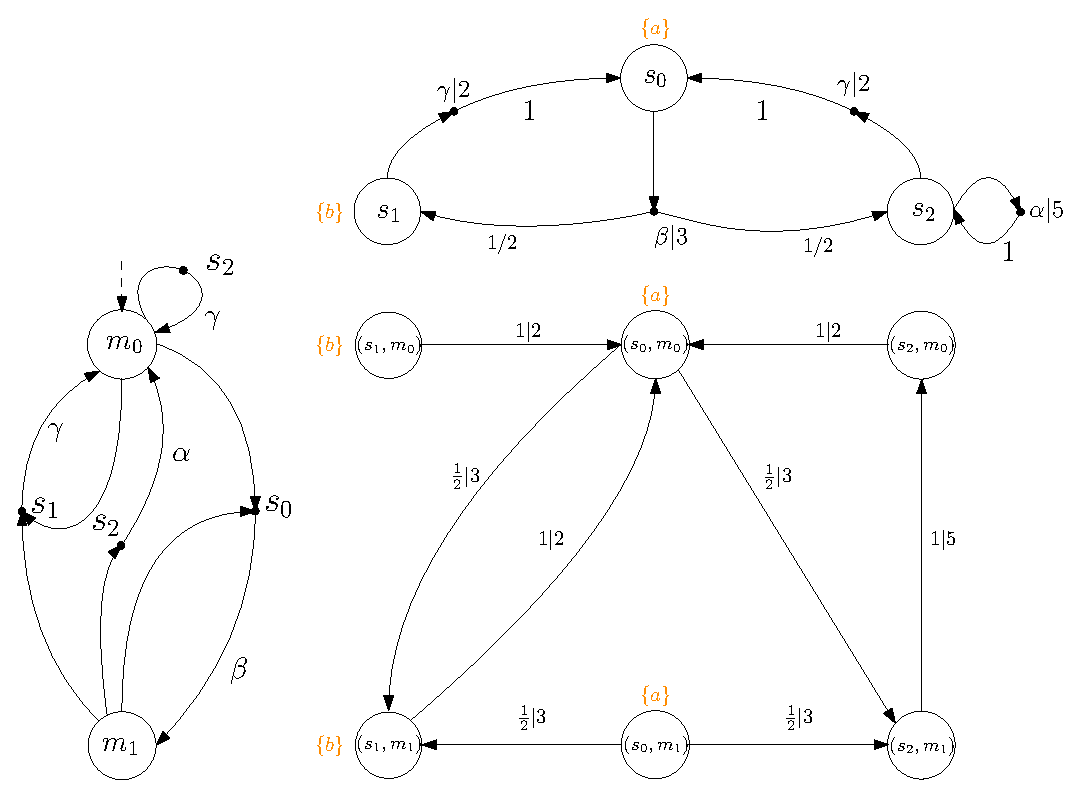
\includegraphics[width=0.55\linewidth]{resources/inductedmarkov}
    \caption{Product of $\mathcal{M}$ by $\sigma$}\label{inducedMC}
  \end{figure}
\end{example}

Finally, the last type of strategy that we will see is a particular case of finite memory strategies, where strategies have only one mode.
In that case, the action chosen by a such strategy only depends on the current state of the system.

\begin{definition}[\textbf{Memoryless strategy}]
  Let $\mathcal{M}=(S, A, \Delta, w, AP, L)$ be an MDP. A \textit{memoryless strategy} is a function
  $
    \sigma: S \rightarrow A
  $ that links each state $s$ of $\mathcal{M}$ to an enabled action $\alpha \in A(s)$ of this state.
\end{definition}

\begin{property}
  A memoryless strategy is a finite memory strategy with only one mode.
\end{property}

\subsection{Objectives in Markov decision processes}
The resolution of problems in MDPs will be done through strategies that will choose the optimal actions to complete different objectives. As for MCs, we will first address the \textit{stochastic reachability problem} in an MDP.
\begin{definition}[\textbf{SR problem}]
  Let $\mathcal{M}=(S, A, \Delta, w, AP, L)$ be an MDP, $s \in S$ be a state of $\mathcal{M}$, $T$ be a set of target states and $\alpha \in [0, 1]$ be
  a probability threshold. The \textit{stochastic reachability} (SR) problem consists
  of deciding if a strategy $\sigma$ exists such that
  \[
    \mathbb{P}_s^\sigma(\Diamond T) \geq \alpha
  \]
\end{definition}

\begin{theorem}
  The SR-problem can be decided in polynomial time in the size of $\mathcal{M}$
  through a linear program, by building a pure memoryless strategy that gives the optimal actions to reach $T$ from every state $s \in S$ (cf. appendix \ref{app-sr} for more details).
\end{theorem}

Before introducing the following, we will first introduce the \textit{truncated sum} of paths of MDPs in order to compute the cost of paths of an MDP.

\begin{definition}[\textbf{Truncated sum for MDPs}]
	Let $\mathcal{M} = (S, A, \Delta, w, AP, L)$ be an MDP, $s \in S$ be a state of $\mathcal{M}$, $T \subseteq S$ be a set of target states and
	$\pi = s_0 \xrightarrow{\alpha_1} s_1 \xrightarrow{\alpha_2} s_2 \xrightarrow{\alpha_3} \dots \in Paths(s)$ be a path of
	$\mathcal{M}$ starting from $s$. The truncated sum $TS^T: Paths(s)
	\rightarrow \mathbb{N} \cup {\infty}$ of the path $\pi$ is defined as follows:
	\[
		TS^T(\pi) =
		\begin{cases}
			\sum_{i = 1}^{n} w(\alpha_i) & \quad \text{if } \forall i \in \{0, \dots, n - 1\}, s_i \notin T \text{ and } s_n \in T \\
			\infty & \quad \text{else, if $ \forall i \in \mathbb{N}, \, s_i \not\in T$}
		\end{cases}
	\]

\end{definition}

By considering the cost of paths of an MDP, we are now interested by building
strategies inducing the shortest path to go from one state to a set of target
states. The notion of shortest path in an MDP is not as obvious as in a graph due to the uncertainty linked to the stochastic environment.
The stochastic shortest path problem in an MDP can be approached in different
ways. We will first approach the \textit{stochastic shortest path expectation} problem and
then approach the \textit{stochastic shortest path percentile} problem. \\

Since events of any MDP controlled by strategy is measurable and
since the cost of paths of any MDP is computable via the truncated sum function, we can
compute the expected length of paths that reach a set of target states using a strategy and, more particularly, build the strategy that will minimise the expected length of these paths.

\begin{definition}[\textbf{SSP-E problem}]
Let $\mathcal{M}=(S, A, \Delta, w, AP, L)$ be an MDP, $s \in S$ be a state of $\mathcal{M}$,
$T \subseteq S$ be a set of target states and $l \in \mathbb{N}$ be a paths length
threshold. The \textit{stochastic shortest path expectation} (SSP-E) problem
consists of deciding if a strategy $\sigma$ exists such that
\[
  \mathbb{E}^\sigma_s(\Diamond T) \leq l
\]
% i.e., if there exists a strategy $\sigma$ such that the expected length of paths starting in the state $s$ in the MC induced by this strategy is lower than the length threshold $l$.
where $\mathbb{E}_s^\sigma(\Diamond T)$ corresponds to the expected cost of paths starting from $s$ in the MC induced by $\sigma$.
\end{definition}

\begin{theorem}
  The SSP-E problem can be decided in polynomial time in the size of $\mathcal{M}$, through a linear program by building a pure memoryless strategy that gives the optimal actions to minimise the expected cost of paths to reach $T$ from every state $s \in S$ (cf. appendix \ref{app-sspe} for more details).
\end{theorem}

Finally, the last problem that we will present in this chapter is the
\textit{stochastic shortest path percentile} problem. For this problem, we will
be interested to decide if there exists a strategy that allows to reach a set of target states with
a cost bounded and an high probability threshold.

\begin{definition}[\textbf{SSP-P problem}]
  Let $\mathcal{M} = (S, A, \Delta, w, AP, L)$ be an MDP, $s \in S$ be a state of
  $\mathcal{M}$, $T \subseteq S$ be a set of target states, $l \in \mathbb{N}$
  be a paths length threshold and $\alpha \in [0, 1]$ be a probability
  threshold. The \textit{stochastic shortest path percentile} (SSP-P) problem
  consists of deciding if there exists a strategy $\sigma$ such that
  \[
    \mathbb{P}_s^\sigma (\Diamond_{\leq l} T) \geq \alpha
  \]
\end{definition}

\begin{theorem}
  The SSP-P problem can be decided in pseudo-polynomial time in the size of $\mathcal{M}$ and $l$ by building a pure finite memory strategy. This strategy is built by unfolding the MDP $\mathcal{M}$ from the state $s$ until $l$ and by resolving the SR problem on this unfolded MDP.
\end{theorem}

\begin{definition}[\textbf{Unfolded MDP until a bounded length}] Let
  $\mathcal{M} = (S, A, \Delta, w, AP, L)$ be an MDP, $s^* \in S$ be a state of
  $\mathcal{M}$, $T \subseteq S$ be a set of target states of $\mathcal{M}$ and $l \in \mathbb{N}$ be a paths length threshold.
  Unfolding $\mathcal{M}$ from $s^*$ until $l$ can be done as follows: \\
  We build $\mathcal{M}_l = (S_l, A_l, \Delta_l, w, AP, L_l)$ for the subset $T_l \subseteq S_l$ where
  \begin{itemize}
  \item $S_l$ is composed of states $(s, v)$ where $s \in S$ et $v \in \{0, \dots, l\} \cup \{\bot\}$.
  We consider that $\bot > l$, with $\bot + v = \bot$ for all $v \in \{0, \dots, l\}$.
  Intuitively, $v$ records the cost of paths while unfolding $\mathcal{M}$.
  As we unfold $\mathcal{M}$ from $s^*$, we have that
  $(s, 0) \not \in S_l$ for all $s \in S$ such that $s \neq s^*$.
  \item For each $\alpha \in A$, we have that $\alpha \in A_l$ and for all $(s, v) \in S_l$, $A_l(s, v) = A(s)$.
  \item $\Delta_l: S_l \times S_l \rightarrow [0, 1]$ is the probability transition function given by:\\
  $\text{Forall } (s, v), (s', v') \in S_l \text{ and for all } \alpha \in A(s),$
  \[
  \Delta_l((s, v), \alpha, (s', v')) =
  \begin{cases}
  	\Delta(s, \alpha, s') & \quad \quad \text{ if } v' = v + w(\alpha) \leq l \text{ or}\\
  	 & \quad \quad \text{ if } v' = \perp \text{ and } v+w(\alpha) > l \\
  	0 & \quad \quad \text{ else}
  \end{cases}
  \]
  \item $L_l:S_l \rightarrow AP \mapsto L_l((s, v)) = L(s)$.
  \item Target states are states of
  $T_l = \{(s, v) \;|\; s \in T \wedge v \leq l \}$.
  \end{itemize}
  \textit{Remark}: since all state $(s, v) \in S_l$ such that $v = \bot$ can never reach $T_l$, it is not useful to keep these states in the unfolded MDP $\mathcal{M}_l$. So, we can replace all these states in $S_l$ with a unique state $\bot$ such that, for all $(s, v) \in S_l$ such that $v \neq \bot$ and for all $\alpha \in A(s)$ such that $v + w(\alpha) > l$,
  $\Delta_l((s, v), \alpha, \bot) = 1$. Then, we define a new action $\alpha_\bot \in A_l$ with an arbitrary weight that will allow a self-loop for $\bot$, i.e., $\Delta_l(\bot, \alpha_\bot, \bot)=1$.
\end{definition}

\begin{example}[\textit{Unfold an MDP}]
  Let $\mathcal{M} = (S, A, \Delta, w, AP, L)$ be the MDP of the example \ref{simple-mdp}.
  This MDP can be unfolded from the state $s_0$ until the threshold $l = 8$ for the target states set $\{s_1\}$ (cf. figure \ref{unfolding}).
  \begin{figure}[h!]
    \centering
    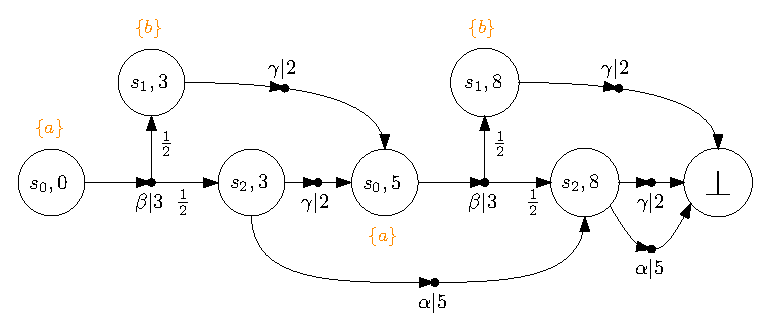
\includegraphics[width=0.8\linewidth]{resources/unfolding}
    \caption{$\mathcal{M}$ unfolded from $s_0$ until $l=8$ for $\{s_1\}$}\label{unfolding}
  \end{figure}
  The highlighted strategy in the figure \ref{unfolding} is the memoryless strategy that resolves the SR problem in $\mathcal{M}_l$. This strategy is the
  same as the one that resolves the SSP-P problem in $\mathcal{M}$ and is thus finite memory in $\mathcal{M}$.
\end{example}

\chapter{Storm overview}
\textit{This chapter is based on the article named ``A Storm is coming : a modern probabilistic model checker'' \cite{storm1} and on the documentation of the tool.} \\

Storm is a probabilistic model checker recently released. It is able to analyse
four Markov models, featuring discrete-time Markov chains and Markov decision processes. The main aim of this tool is to be competitive in terms of performances, to be updated with new verification algorithms, to be able to
deal with a large panel of modeling languages,... This tool provides %many other
a lot of model checking features, including solvers for problems presented in the previous chapter and
for multi-objective problems.

\section{Models}
As mentioned above, Storm allows to model-check four types of Markov models.
The first family of models contains discrete-time Markov models that are covered in the first chapter, composed by
discrete time Markov chains and Markov decision processes.
The second family of models contains continuous-time Markov models, composed by continuous time Markov chains and Markov automata.
\subsubsection*{Continuous time Markov chains (CMC)}
These models are similar to discrete time Markov chains but each state $s$ is
characterised by an exit rate $\lambda_s$.
The time $t$ spent in each state $s$ of the system is negatively exponentially distributed with this rate, i.e., $e^{- \lambda_s t}$.
This exit rate and a probability transition function allow to induce a generator
function with which it is possible to compute the probability
%to go from one state to another after a certain time.
that the system is currently in a state $s'$ while the system was in the state $s$, $t$ time units ago. Note that there is no more ``step'' notion in continuous
Markov model types.
\subsubsection*{Markov automata (MA)}
This is a continuous nondeterministic Markov model. The key idea is the same that between MCs and MDPs in discrete time. \\

We will not dwell on continuous time models anymore and focus primarily on discrete time models.

\section{Input formats}
Storm supports various native input formats, including Prism, Jani, generalised stochastic Petri nets, dynamic fault trees, cpGCL and explicit format.
We will introduce some of these input languages by presenting how to use them to modelize our
discrete time models.
\subsection{Prism}
The Prism language \cite{prismsynt} allows to deal with MCs, CMCs and MDPs in Storm.
It is a state-based language using reactive modules.
We will not define the complete syntax and semantic of Prism but rather provide a way to
define our MDPs using this language. Let $\mathcal{M} = (S, A, \Delta, w, AP, L)$ be a MDP such that the state space
$S$ is finite, with $|S| = n$, and $i \in \{0, \dots, n-1\}$ such that $s_i \in S$ is the $i^{\text{th}}$ state of $S$ from which events that we are
interested to measure start. \\

In Prism language, a \textit{module} represents a component of the system.
Depending on how our MDPs are defined, we just need a single module to
represent them. A module allows to characterise $S$, $A$ and $\Delta$. We begin by enumerating states of $\mathcal{M}$ :
\[
  s: [0\, ..\, n-1] \; \text{init} \; i;
\]
In this manner, we express that for all $j \in \{0, \dots, n-1\}$, $s_j \in S$
is the $j^{\text{th}}$ state of $S$ and $s_i$ is the initial state from which events start. In Prism language, $s$ is considered as a \textit{variable} of the module, ranging on states of $\mathcal{M}$. Note that a variable represents a set of states of the MDP. Thus, it is possible that a module have more than one variable if the state space of the MDP is formed by more than one sates set.
Thanks to variables of the system, it is possible to form predicates $\Phi$ with the following  syntax :
\begin{align*}
  \Phi &::= true \; | \; s \varphi x \; | \; (X) \; | \; (\Psi) \\
  X &::= \Phi \; | \; \Phi \& X \\
  \Psi &::= \Phi \; | \; \Phi || \Psi
\end{align*}
where $s$ is a variable of the module, $\varphi \in \{<, \leq, >, \geq, =, \neq\}$
and $x \in \mathbb{N}$. Let $s^* \in S$ be a state of $\mathcal{M}$. We have that $s^* \models \Phi$ iff $\Phi$ is true for the state $s^*$, i.e.,
\begin{itemize}
  \item $s^* \models true$,
  \item $s^* \models s \varphi x$ iff there exists a $j \in \mathbb{N}$ in the range of indices of the module variable $s$ by which the state $s^*$ is represented (i.e., $s^*$ is represented by $s=j$) such that $j \varphi x$.
  \item $s^* \models (\Phi_1 \& \dots \& \Phi_m)$ iff
    for all $k \in \{1, \dots, m\}$, $s_j \models \Phi_k$, and
  \item $s^* \models (\Phi_1 || \dots || \Phi_m)$ iff
    there exists $k \in \{1, \dots, m\}$ such that $s \models \Phi_k$.
\end{itemize}
We denote by $Sat(\Phi)$ the set of states that satisfies the predicate $\Phi$, i.e., $Sat(\Phi) = \{s \in S \; | \; s \models \Phi\}$. \\

The behaviour of the module, i.e., transitions of $\{ (s, \alpha, s') \in S \times A \times S \; | \; \Delta(s, \alpha, s') > 0 \}$, is then described
inside the module by a set of \textit{guarded commands}, taken the following form :
\[
  [\alpha] \; \Phi \rightarrow \delta_1 : \phi_1 + \dots + \delta_m : \phi_m;
\]
where $\Phi$ is a predicate such that for all $s \in Sat(\Phi)$, $\alpha \in A(s)$, $\delta_k \in [0, 1]$ and $\phi_k$ is an \textit{update formula} describing a state represented by a variable of the module. This guarded command basically means that all states that satisfy the predicate $\Phi$ go to the state  described by $\phi_k$ with a probability $\delta_k$, where the action $\alpha$ is chosen.
An update formula $\phi$ is of the form :
\[\phi::=(x'_1=u_1) \& (x'_2=u_2) \& \dots \& (x'_k=u_k)\]
where $x_1, x_2, \dots, x_k$ are variables of the module and $u_1, u_2, \dots, u_k$ are expressions over all variables.
% \begin{align*}
%   \phi &::= (s'=\chi) \; | \; (s'= \mu(\chi, \chi)) \; | \; \psi \\
%   \chi &::= s \varphi x \; | \; x \\
%   \psi &::= \phi \; | \; \phi \& \psi
% \end{align*}
% where $s$ is a variable of the module,
% $\varphi \in \{+, -\}$, $\mu \in \{\min, \max \}$ and $x \in \mathbb{N}$.
% Let assume that the system is currently in the $j^\text{th}$ state of $S$, i.e.,
% in the state $s_j$
% %The expression $\chi$ actually represents the core of a variable update ; it represents the index of the state to which the system evolves.
% %\begin{itemize}
% %  \item $\chi = x$ directly refers to the index $x$ of the variable to update and
% %  \item $\chi = s \varphi x$ refers to the current index of the variable $s$ on which the operation $\varphi x$ is applied (here, $j \varphi x$).
% %\end{itemize}
% and let $k \in \{0, \dots, n-1\}$. We have that $s_k \models \phi$ iff $\phi$ refers to the state $s_k$, i.e.,
% \begin{itemize}
%   \item $s_k \models s' = x$ iff $k = x$. Then the system go from $s_j$ to $s_x$.
%   \item $s_k \models s' = s \varphi x$ iff $k$ is the current index of the variable $s$ on which the operation $\varphi$ has been applied. Here, we have $k = j \varphi x$. Thus the system go from $s_j$ to $s_{j+\varphi}$.
% \end{itemize}
More specifically, transitions of $\mathcal{M}$ can be described with the following guarded command :
let $s_j$ be the $j^{\text{th}}$ state of $S$, for all enabled actions $\alpha \in A(s_j)$ of $s_j$,
\[
  [\alpha] \; s=j \rightarrow \delta_0 : s'=j_0 + \dots + \delta_{m-1} :  s'=j_{m-1};
\]
where $s_{j_0}, \dots, s_{j_{m-1}}$ are $\alpha$-successors of $s_j$ and $\delta_k = \Delta(s_j, \alpha, s_{j_k})$,
with  $m=|Succ(s_j,\alpha)|$, $k \in \{0, \dots, m-1\}$, $j_k \in \{0, \dots, n-1\}$ and $s_{j_k}$, the $k^\text{th}$ $\alpha$-successor of $s_j$ and the $j_k^\text{th}$ state of $S$. \\

The set of atomic propositions $AP$ and the labelling function $L$ of $\mathcal{M}$ are characterised in Prism language as follows : for all $a \in AP$,
\[
  \text{label} \; ``a" = \Phi;
\]
such that the set of states that satisfy the predicate $\Phi$ is actually the set $\{ s \in S \; | \; a \in L(s) \}$. \\

% \[
%   \text{label} \; ``a" = (s=j_0\, \& \, \dots \, \& \, s=j_{m-1});
% \]
% where $S_a= \{s \in S \; | \; a \in L(s) \}$ and $s_{j_k} \in S_a$,
% with $m = |S_a|$, $k \in \{0, \dots, m-1\}$,
% $j_k \in \{ 0, \dots, n-1 \}$ and $s_{j_k}$, the $k^\text{th}$ state of $S_a$ and the $j_k^\text{th}$ state of $S$.
%

Finally, the weight function $w$ can be characterised with the notion of \textit{rewards}. In Prism language, it is possible to associate to each transition
of the set $\{ (s, \alpha, s') \in S \times A \times S \; | \; \Delta(s, \alpha, s') > 0 \}$ a real value. In Prism language, a \textit{dimension rewards} is a set of rewards that take the following form:
\[
  [\alpha] \; \Phi : x;
\]
where $\alpha \in A$ is an action, $\Phi$ is a predicate and $x \in \mathbb{R}$
is the value of the reward of going from a state $s \in S$, such that $\alpha \in A(s)$, to states of $Sat(\Phi)$. Note that if the action $\alpha$ is omitted (giving a reward of the form $[]\; \Phi : x^*;$), each transition $(s, \alpha, s') \in S\times A \times S$ such that $s \in Sat(\Phi)$ and $\alpha \in A(s)$
has a reward of $x^*$. Note also that it is possible to specify multiple dimension rewards for a MDP. We will detail this notion later.
We can adapt the reward notion to describe the weight function of our MDPs with a set of rewards formed as follows:
let $\alpha \in A$ be an action of $\mathcal{M}$ and $x = w(\alpha)$, the reward $x$ formed by
\[
  [\alpha] \; true : x;
\]
is actually the cost of the action $\alpha$.

\begin{example}[\textit{Define an MDP in Prism language}]
Let $\mathcal{M}=(S, A, \Delta, w, AP, L)$ be the MDP of the figure \ref{prism-simple}. This MDP can be defined in Prism language as follows:\\
\begin{minipage}{0.4\linewidth}
  \lstinputlisting[language={Prism},
      rulesepcolor=\color{black}, rulecolor=\color{black}, breaklines=true,
      breakatwhitespace=true, firstnumber=1, firstline=1, lastline=25]{resources/simple_mdp.prism}
\end{minipage}
\begin{minipage}{0.6\linewidth}
    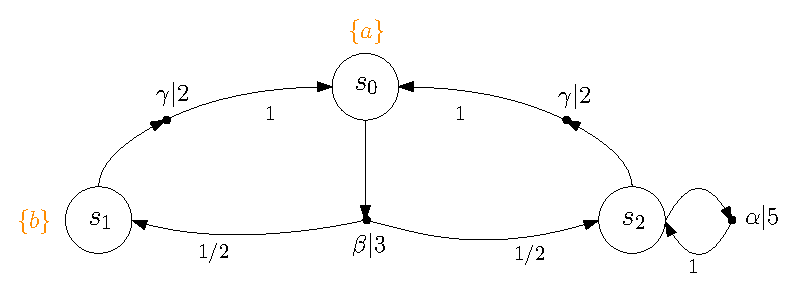
\includegraphics[width=\linewidth]{resources/simple-mdp}
    \captionsetup{justification=centering}
    \captionof{figure}{MDP $\mathcal{M}$, with $S = \{s_0, s_1, s_2\}$, $A = \{\alpha, \beta, \gamma\}$ and $AP = \{a, b\}$}\label{prism-simple}
\end{minipage}
\end{example}

\begin{example}[\textit{Unfold an MDP in Prism language}]
Let $\mathcal{M}=(S, A, \Delta, w, AP, L)$ be the MDP of the figure \ref{prism-simple}, $s \in S$ be a state of $\mathcal{M}$ and $l \in \mathbb{N}$
be a length threshold such that $l=8$. We can define the unfolding of $\mathcal{M}$ until $l$ for the set of target states $T = \{s_1\}$ (cf. figure \ref{unfolding}) in Prism language as follows:
\lstinputlisting[language={Prism},
    rulesepcolor=\color{black}, rulecolor=\color{black}, breaklines=true,
    breakatwhitespace=true, firstnumber=1, firstline=1, lastline=25]{resources/unfolded_simple_mdp.prism}
\end{example}
Since the state space of the unfolded MDP $\mathcal{M}_l$ is a Cartesian product between the state space $S$ of $\mathcal{M}$ and the set $V = \{0, \dots, l, \bot\} \subseteq \mathbb{N} \cup \{\bot\}$, we can define the variables of the unfolded MDP $\mathcal{M}_l$ with the variables of the MDP and a new variable $v$, ranging from $0$ to $l+1$ (where the $(l+1)^\text{th}$ state actually represents the $\bot$ value). The guarded
commands of the module are obviously defined, following the definition of the
probability transition function $\Delta_l$ of any unfolded MDP. Finally, a label $target$ is added,
labelling each state of the set $T_l = \{ (t, v) \in S \times V \; | \; t \in T \; \wedge \; v \leq l \}$.

\chapter{Model checking for Markov decision processes}

Storm allows to model-check discrete-time and continuous-time models, i.e.,
verify that properties hold in states of models. This
chapter will cover discrete-time model checking via a \textit{probabilistic branching-time logic}. We will detail the syntax, the semantic and model checking algorithms of this logic.
We will see that it is possible to extend this logic to support weights of MCs and MDPs. Then, we will see that it is
possible to formulate requests with this logic to solve
problems we encountered in the first chapter and that we
will address in the following chapter, covering multi-objective support for MDPs. \\

As model checking for MDPs uses the notion of strategy to resolve nondeterminism,
we first need to introduce the probabilistic branching time logic for MCs.

\section{Probabilistic computational tree logic}
\textit{Probabilistic computational tree logic} (or \textbf{PCTL}, for short) is a \textit{branching-time temporal logic}.
This logic allows to verify probabilistic systems via an
%probabilistic
execution tree, actually named \textit{computational tree}. For a given system, this tree consists of an infinite unfolding of this system, considering
all branching possibilities.
%Thus, it is actually an MC with an infinite tree as underlying graph.
The key idea of this tree is that each branch of a node leads to a possible future of this node.
So, this tree is highly linked to cylinder sets.  Possible futures of a node actually correspond to paths of the cylinder set for which the prefix leads the root to the node in the tree.
\begin{example}[\textit{Computational tree of an MC}]
Let $\mathcal{M}$ be the MC of the figure \ref{ct1}. The computational tree of $\mathcal{M}$ starting from the state $s_0$ is
given in the figure \ref{ct2}. We clearly see in this tree that each possible future of a node $s^*$ actually corresponds to a state $s'_n$ of a path $\pi = s'_0 \dots s'_k \dots s'_n \dots \in Cyl(s'_0 \dots s'_k)$ such that $s'_0 = s_0$, $s'_k=s^*$ and $k < n$.
For example, $s_1$ is a possible future of the node $s_0$ (for which the prefix is $s_0s_0$ in the tree) because the path $\pi = s_0s_0s_0(s_1s_2)^\omega$ is in $Cyl(s_0s_0)$.
\begin{figure}[h]
  \begin{minipage}{0.4\linewidth}
    \centering
    
\includegraphics[width=0.8\linewidth]{resources/CLT_unfolding_1}
    \captionsetup{justification=centering}
    \captionof{figure}{MC $\mathcal{M}$ with $3$ states, $s_0, s_1$ and $s_2$, and $2$ atomic propositions, $a$ and $b$}\label{ct1}
  \end{minipage}
  \begin{minipage}{0.6\linewidth}
    \centering
    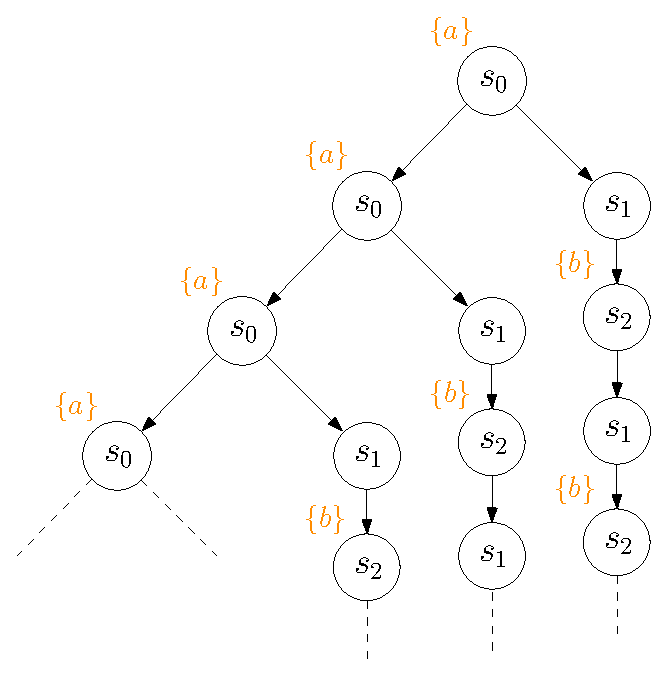
\includegraphics[width=0.8\linewidth]{resources/CLT_unfolding_2}
    \captionsetup{justification=centering}
    \captionof{figure}{Computational tree of $\mathcal{M}$ starting from $s_0$}\label{ct2}
  \end{minipage}
\end{figure}
We will see that it is possible to express formulae in PCTL describing states properties of the system like the following one:
\begin{center}
``\textit{Do all executions starting from the state $s_0$ always eventually reach $b$ with a nonzero probability ?}''
\end{center}
Model checking algorithms of PCTL will answer \textit{yes} to this.
Intuitively, if we refer to the computational tree,
%we see that it is possible to reach a node labeled with $b$,
%from any node of the tree,
%via a path from this node that has a nonzero probability.
%we see that it is possible to reach a node labelled with $b$ from any node of the tree and, each cylinder set
%for which the prefix leads the root to any node has a nonzero probability:
we see that a node labelled with $b$ appears in the future of any node $s^*$ of the tree. Furthermore, there exists an index $n$ for each path $\pi = s'_0 s'_1 s'_2 \dots s'_n \dots \in Cyl(s'_0 \dots s'_k)$, where $s'_0 \dots s'_k$ is the prefix that leads the root to the node $s^* = s'_k$ in the tree, such that $k <n$ and $s'_n$ is labelled with $b$, except for the path $s_0^\omega$ (corresponding to the left path in the computational tree).
Since this path has a zero probability, we have that this property is verified with a probability one from the state $s_0$.
We will see in this chapter how to verify formally each property of this type.
%let $\hat{\pi} = s'_0 \dots s'_n$ be a finite path of $\mathcal{M}$, starting from the state $s_0$ of $\mathcal{M}$ and referring to a finite path starting from the root of the tree. If there exists an index $k$, such that $1 \leq k \leq n$ and $s'_k = s_1$, then $\mathbb{P}_{s_0}(Cyl(s'_0 \dots s'_k \dots s'_n)) = \prod_{i=0}^{k-1} \Delta(s'_i, s'_{i+1}) \cdot 1^\omega = \frac{1}{10}^{k-1}$.
%Else, $\hat{\pi} = s_0^{n+1}$ and $\mathbb{P}_{s_0}(Cyl(s_0^{n+1})) = \frac{1}{10}^n$.
%Furthermore, all executions starting from $s_0$ has a probability one to always eventually reach a state labeled with $b$: the only path starting from $s_0$ that does not allow it is the path $s_0^\omega$ (corresponding to the left path in the computational tree) and has a zero probability.
\end{example}

\subsection{Syntax and semantic}
PCTL has a two stages syntax where PCTL formulae are classified into state and path formulae. Intuitively, \textit{state formulae} are assertions about atomic propositions in a state $s$ and about probabilities over their branching structure, i.e., probabilities of \textit{path formulae} starting from $s$. Actually, a path formula will impose conditions on a set of paths and this path formula will be quantified
by probability bounds.

\begin{definition}[\textbf{Syntax of PCTL}]
Let $AP$ be a set of atomic propositions,
\begin{itemize}
  \item PCTL \textit{state formulae} are formed according the following grammar:
  \[
    \Phi ::= true \;\; | \;\; a \;\; | \;\; \Phi_1 \wedge \Phi_2 \;\; | \;\; \neg \Phi \;\; | \;\; \mathcal{P}_J(\phi)
  \]
  where $a \in AP$ is an atomic proposition, $J \subseteq [0, 1]$ gives probability bounds and $\phi$ is a path formula.
  \item PCTL \textit{path formulae} are formed according the following grammar:
  \[
  \phi ::= \bigcirc \Phi \;\; | \;\; \Phi_1 \U \Phi_2 \;\; | \;\; \Phi_1 \U^{\leq n} \Phi_2
  \]
  where $\Phi$, $\Phi_1$ and $\Phi_2$ are state formulae and $n \in \mathbb{N}$.
\end{itemize}
\end{definition}
Intuitively, $\mathcal{P}_J(\phi)$ specify that the probability of paths satisfying the path formula $\phi$ must be in the interval $J$. A path formula is formed by temporal operators, like $\bigcirc$ and $\U$, with $\U^{\leq n}$ being $\U$ bounded by a maximum number of steps.  There exists some other linear temporal operators, dealing with paths of the system (cf. figure \ref{ltl}). These operators can be derived from the PCTL grammar:
let $J \in [0, 1]$ giving probability bounds, $\Phi$ be a state formula and $n \in \mathbb{N}$ be a number of steps,

\makeatletter
\newcommand*\bigcdot{\mathpalette\bigcdot@{.5}}
\newcommand*\bigcdot@[2]{\mathbin{\vcenter{\hbox{\scalebox{#2}{$\m@th#1\bullet$}}}}}

\makeatother
\begin{flalign}
  &\bigcdot \; \mathcal{P}_J(\Diamond \Phi) \equiv \mathcal{P}_J(true \U \Phi) \tag{\textit{eventually} probability} \\
  &\bigcdot \; \mathcal{P}_J(\Diamond^{\leq n} \Phi) \equiv \mathcal{P}_J(true \U^{\leq n} \Phi) \tag{\textit{bounded enventually} probability} \\
  &\bigcdot \; \mathcal{P}_J(\Box \Phi) \equiv
    \neg \mathcal{P}_J(\Diamond \neg \Phi)
    \tag{\textit{always} probability}
\end{flalign}

\begin{figure}[h]
  \centering
  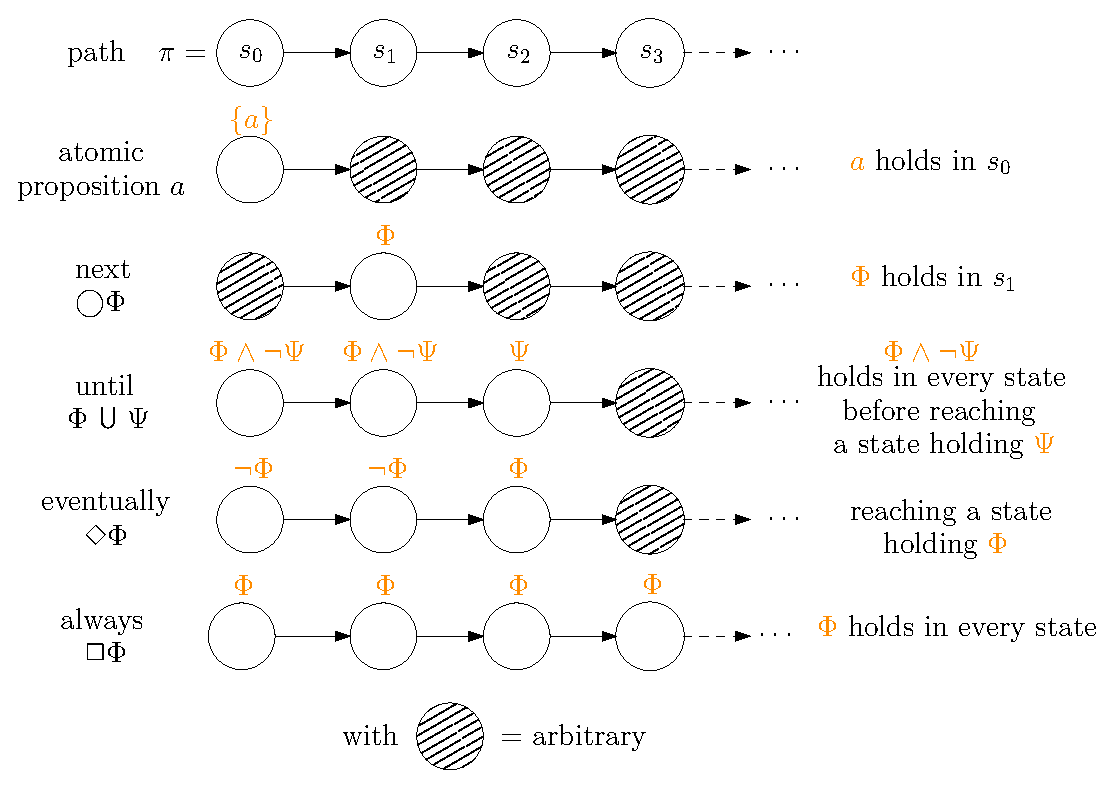
\includegraphics[width=0.85\linewidth]{resources/LTL}
  \caption{Intuitive semantic of linear temporal operators}\label{ltl}
\end{figure}

\begin{definition}[\textbf{Semantic of PCTL}]
  Let $\mathcal{M} = (S, \Delta, AP, L)$ be an MC and $s \in S$, be a state of $\mathcal{M}$,
  \begin{flalign*}
  \intertext{$s \models \Phi$ iff the state formula $\Phi$ holds in the state $s$, i.e.,}
    &\bigcdot\; s \models true, &&&\\
    &\bigcdot\; s \models a &\text{ iff }& a \text{ is a label of $s$, i.e., } a \in L(s),&\\
    &\bigcdot\; s \models \Phi_1 \wedge \Phi_2&\text{ iff }& s \models \Phi_1 \text{ and } s \models \Phi_2,&\\
    &\bigcdot\; s \models \neg \Phi &\text{ iff }& s \not\models \Phi, &\\
    &\bigcdot\; s \models \mathcal{P}_J(\phi) &\text{ iff }& \mathbb{P}_s(\{ \pi \in Paths(s) \; | \; \pi \models \phi \}) \in J.& \\
  \intertext{Following a path $\pi = s_0s_1s_2\dots \in Paths(s)$, $\pi \models \phi$ iff $\pi$ satisfies the path formula $\phi$, i.e., }
  &\bigcdot\;\pi \models \Phi&\text{ iff }&s_0 \models \Phi,&\\
  &\bigcdot\;\pi \models \bigcirc\, \Phi&\text{ iff }&s_1 \models \Phi,&\\
  &\bigcdot\;\pi \models \Phi_1 \U \Phi_2 &\text{ iff }& \exists j \in \mathbb{N},\, s_j \models \Phi_2
    \text{ and } \forall i \in \mathbb{N}, \, i < j, \, s_i \models \Phi_1,&\\
  &\bigcdot\;\pi \models \Phi_1 \U^{\leq n} \Phi_2 &\text{ iff }& \exists j \in \mathbb{N}, \, j \leq n ,\, s_j \models \Phi_2
    \text{ and } \forall i \in \mathbb{N}, \,i < j, \, s_i \models \Phi_1.&\\
  \intertext{Additionally,}
  &\bigcdot\; \pi \models \Diamond \Phi&\text{ iff }& \exists j \in \mathbb{N}, \, s_j \models \Phi,&\\
  &\bigcdot\; \pi \models \Box \Phi&\text{ iff }& \forall j \in \mathbb{N}, \, s_j \models \Phi.&
  \end{flalign*}
\end{definition}
\begin{remark}[\textit{Measurability of path formulae}]
Since $\mathcal{P}_J(\phi)$ refers to probabilities, $\neg \mathcal{P}_J(\phi) = \mathcal{P}_{J'}(\phi)$ for any path formula $\phi$, with $J'=[0, 1] \setminus J$. Then, the event $\{ \pi \in Paths(s) \; | \; \pi \models \phi\}$ must be measurable to verify that $\mathcal{P}_J(\phi)$ holds in any state. We will see that these events can be formed through countable unions of cylinder sets, ensuring their measurability.
\end{remark}
\begin{remark}[\textit{Probabilistic satisfiability of path formulae}]
Let $\mathcal{M}$ be the MC of the figure \ref{pctlctl}.
\begin{figure}[h]
  \centering
  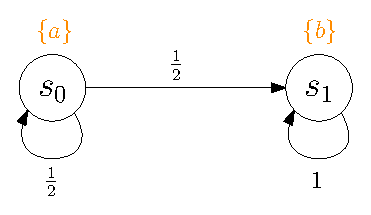
\includegraphics[width=0.25\linewidth]{resources/PCTL_CTL}
  \captionsetup{justification=centering}
  \caption{MC $\mathcal{M}$ with $2$ states, $s_0$ and $s_1$, and $2$ atomic propositions, $a$ and $b$}\label{pctlctl}
\end{figure}
\begin{itemize}
% \item Let assume that there exists a path $\pi \in Paths(s_0)$ starting from $s_0$ in $\mathcal{M}$ such that $\pi \not \models \phi$, for any PCTL path formula $\phi$. That does not mean that $s_0 \models \mathcal{P}_{<1}(\phi)$: take $\pi=s_0^\omega$ and $\phi = \Diamond b$, we have that $s_0^\omega \not \models \Diamond b$ and $\mathbb{P}_s(\Diamond \{s_1\}) = 1$.
% Then $s_0 \models \mathcal{P}_{=1}(\Diamond b)$.
  \item Let assume there exists a state $s$ in an MC such that $s \models \mathcal{P}_{=1}(\phi)$, for any path formula $\phi$. That does not mean that all paths $\pi \in Paths(s)$ satisfy $\phi$, i.e.,
  \[s \models \mathcal{P}_{=1}(\phi) \centernot\implies \forall \pi \in Paths(s), \, \pi \models \phi.\]
  Indeed, consider the MC $\mathcal{M}$ and take the state $s_0$ of $\mathcal{M}$, the path $s_0^\omega \in Paths(s_0)$ and the path formula $\Diamond b$. We have $s_0 \models \mathcal{P}_{=1}(\Diamond b)$, because $\mathbb{P}_{s_0}(\Diamond \{s_1\})=1$, but we have $s_0^\omega \not \models (\Diamond b)$.

  \item Let assume there exists a state $s$ in an MC such that there exists a path $\pi \in Paths(s)$ starting from this state $s$ such that $\pi \models \phi$ for any path formula $\phi$.
  That does not mean that $s \models \mathcal{P}_{> 0}(\phi)$, i.e.,
  \[
    \exists \pi \in Paths(s),\, \pi \models \phi \centernot\implies s \models \mathcal{P}_{>0} (\phi).
  \]
  Indeed, consider the MC $\mathcal{M}$ and take the state $s_0$, the path $s_0^\omega \in Paths(s_0)$ and the path formula $\Box a$. We have that the path $s_0^\omega$ is the only path of $\mathcal{M}$ that verifies $\Box a$ (and thus, $s_0^\omega \models \Box a$).
  However, we have $\mathbb{P}_s(\{s_0^\omega\})=0$. Then, $s_0 \models \mathcal{P}_{=0} (\Box a)$.
\end{itemize}
\end{remark}

\begin{definition}[\textbf{Satisfiability set for PCTL}]
  Let $\mathcal{M}=(S, \Delta, w, AP, L)$ be an MC and $\Phi$ be a PCTL state formula on $AP$. The \textit{satisfiability set} for the MC $\mathcal{M}$ is defined as follows:
  \[
    Sat(\Phi) = \{ s \in S \, | \, s \models \Phi \}.
  \]
\end{definition}

\section{Temporal events in Markov chains}\label{tempevent}
In Markov chains, \textit{temporal events} allow to describe \textit{quantitative} and \textit{qualitative} properties.
Quantitative properties may assert the probability to reach a subset of target states, avoiding some bad states in a infinite or finite number of steps, and
qualitative properties are special cases of quantitative properties where probabilities are trivial (i.e., zero or one).
In order to describe these temporal events, we use \textit{LTL-like} notations.
\textit{Linear temporal logic} (LTL) is a logical formalism
that is suited for specifying linear temporal properties.
In PCTL, notations of linear temporal operators (cf. figure \ref{ltl}) are actually derived from LTL temporal operators, dealing with paths of any system.
For example, following a subset of target states $T \subseteq S$ of the system, the event of reaching $T$ is denoted by $\Diamond T$ that is defined with a finite union of cylinder sets, ensuring its measurability.
We will define here some temporal events, that are actually used to form PCTL path formulae events. So, we need to ensure their measurability.
Furthermore, we will present how to compute their probability, which will be useful later to model-check Markov chains and Markov decision processes in PCTL.
\subsection{Constrained reachability}
\begin{definition}[\textbf{Constrained reachability event}]
Let $\mathcal{M}= (S, \Delta, w, AP, L)$ be an MC, $s \in S$ be a state of $\mathcal{M}$ from which events start, $T, C \subseteq S$ and $n \in \mathbb{N}$.
The events $C \U^{\leq n} T$ and $C \U T$ are defined as follows:
\begin{align*}
  C \U^{\leq n} T &= \bigcup_{k=0}^n\,\bigcup_{s_0\dots s_k \in Paths_{fin}^{C,\, k,\, T}(s)} Cyl(s_0\dots s_k),\\
  C \U T &= \bigcup_{k\in \mathbb{N}}\,\bigcup_{s_0\dots s_k \in Paths_{fin}^{C,\, k,\, T}(s)} Cyl(s_0\dots s_k)
\end{align*}
where \[Paths_{fin}^{C,\, n,\, T}(s) = \{ s_0 \dots s_n \in Paths_{fin}(s) \; | \; s_i \in C\;\; \forall i \in \mathbb{N},\, i < n \; \; \wedge s_n \in T\},\]
and $\mathbb{P}_s(C \U^{\leq n} T), \mathbb{P}_s(C \U T)$ actually denote the probability measure of the union of cylinder sets of finite paths  of $Paths_{fin}^{C, \, k, \, T}(s)$ starting from the state $s \in S$.
\end{definition}

The constrained reachability event allows to derivate some other classical events:
\begin{itemize}
  \item $\Diamond T = S \U T$, i.e., \textit{reach $T$} (cf. subsection \ref{obj-MC} in the first chapter),
  \item $\Box T =  \overline{\Diamond \overline{T}} \; \implies \; \mathbb{P}_s(\Box T) = 1 - \mathbb{P}_s (\Diamond (S \setminus T))$, i.e., \textit{always encounter $T$}.
\end{itemize}
So, if we can compute the constrained reachability event probability, then we are able to compute the probability of $\Diamond T$ and $\Box T$ events.
Let $S_{=0}$, $S_{=1}$ and $S_{=?}$ be partitions of $S$ such that
\begin{itemize}
  \item $T \subseteq S_{=1} \subseteq \{s \in S \; | \; \mathbb{P}_s(C \U T) = 1\}$,
  \item $S \setminus (C \cup T) \subseteq S_{=0} \subseteq \{ s \in S \; | \; \mathbb{P}_s(C \U T) = 0 \}$,
  \item $S_? = S \setminus (S_{=1} \cup S_{=0})$.
\end{itemize}
Then, let $A$ be a quadratic matrix with rows and columns referring the states of $S_?$. This matrix is obtained from the transition function $\Delta$ as follows:
\[
  A_{i, j} = \Delta(s_i, s_j) \quad \forall s_i, s_j \in S_?
\]
Let $n_?$ = $|S_?|$. Similarly, let $b$ be a vector of probabilities in $[0, 1]^{n_?}$ , defined as $(b_s)_{s \in S_?}$ such that $b_s = \sum_{t \in S_{=1}} \Delta(s, t)$, i.e., such that $b_s$ describes the probability of reaching a state of $T$ in one outgoing transition of the state $s$.

\begin{notation}[\textit{Lifted probability transition}]
  Let $s \in S$ be a state of $\mathcal{M}$. We denote by $\Delta(s, T)$ the probability of reaching $T$ in one outgoing transition of $s$, i.e., $\Delta(s, T) = \sum_{t \in T} \Delta(s, t)$.
\end{notation}
\noindent So, we have $b_s = \Delta(s, S_{=1})$ for each $s \in S_?$.
\begin{theorem}[\bfseries\itshape Least fixed point characterisation]\label{theoCUT}
  Let $x$ be a vector of probabilities in $[0,1]^{n_?}$ such that $x=(\mathbb{P}_s(C \U T))_{s \in S_?}$. This vector is the
  \textit{least fixed point} of the operator $\Upsilon : [0, 1]^{n_?} \rightarrow [0, 1]^{n_?}$. Let $(y_s)_{s \in S_?} \in [0, 1]^{n_?}$, the least fixed point of the operator $\Upsilon$ is given by
  \[
    \Upsilon(y) = A y + b
  \]
  Furthermore, let $x^{(0)} = \vec{0}$ be the vector consisting of zeros only and $x^{(n+1)} = \Upsilon(x^{n})$ for $n \in \mathbb{N}$, then
  \begin{itemize}
    \item $x^{(n)} = (x_s^{(n)})_{s \in S_?}$, where $x_s^{(n)} = \mathbb{P}_s(C \U^{\leq n} S_{=1})$ for each state $s \in S_?$,
    \item $x^{(0)} \leq x^{(1)} \leq x^{(2)} \leq \dots \leq x$, and
    \item $x = \lim_{n\rightarrow\infty}x^{(n)}$.
  \end{itemize}
  where $\leq$ denotes here the partial order relation \[\leq \,=\, \{ (y, y') \in [0, 1]^{n_?} \times [0,1]^{n_?} \; | \; y_s \leq y'_{s} \;\; \forall s \in S_?\}.\]
\end{theorem}
By definition of $A$ and $b$, for any $s \in S_?$ and for $y = (y_s)_{s \in S_?}$,
\[
  (\Upsilon(y))_s = y_s = \sum_{s' \in S_?} \Delta(s, s') \cdot y_{s'} + \Delta(s, S_{=1}).
\]
Furthermore, let $x_s = \mathbb{P}_s(C \U T)_{s \in S_?}$ for each state $s \in S$, by definition of $\Upsilon$, we have that
\begin{flalign}
  x^{(0)} &= \vec{0}, \notag \\
  x^{(1)} &= A x^{(0)} + b \notag \\
          &= b, \tag{\itshape state of $C$ reaching $S_{=1}$ in one transition}\\
  x^{(2)} &= A x^{(1)} + b \notag \\
          &= A b + b \notag \\
          &= (\sum_{s' \in S_?} \Delta(s, s') \cdot \Delta(s', S_{=1}) + \Delta(s, S_{=1}))_{s \in S_?} \tag{\itshape state of $C$ reaching $S_{=1}$ in max. two transition steps} \\
  &\dots \notag \\
  x^{(n)} &= A x^{(n-1)} + b \tag{\itshape state of $C$ reaching $S_{=1}$ in max. $n$ transition steps} \\
  &\dots \notag \\
  x &= Ax+b \notag \\
  x &= (\sum_{s' \in S} \Delta(s, s') \cdot x_{s'} + \Delta(s, S_{=1}))_{s \in S_?} \tag{\itshape state of $C$ eventually reaching $S_{=1}$}
\end{flalign}
\begin{remark}[\textit{Choosing $S_{=0}$ and $S_{=1}$}]\label{remarkS0S1}
For efficiency reasons, it is a good idea to deal with the largest subsets $S_{=0}$ and $S_{=1}$. Indeed, this allows to reduce
the size of the matrix $A$ and allows faster computations to solve the linear equation defined by $x = Ax + b$.
However, for computational reasons, we need to deal with the largest set $S_{=0}$ as possible, i.e., $S_{=0} = \{ s \in S \; | \; \mathbb{P}_s(C \U T) = 0 \}$. Indeed, for some instance, choosing $S_0 = S \setminus (C \cup T)$ is not sufficient.
Let $\mathcal{M}$ be the MC of the figure \ref{s0s1} and $T = \{t\}$.
\begin{figure}[h]
  \centering
  
\includegraphics[width=0.3\linewidth]{resources/S0S1}
  \caption{Markov chain $\mathcal{M}$ with $2$ states : $s$ and $t$}\label{s0s1}
\end{figure}
Consider the event $\Diamond T$. Let take the smallest subsets $S_{=1} = T$ and $S_{=0} = S \setminus (S \cup T) = \emptyset$, thus $S_? = S \setminus T = \{s\}$. Following the theorem \ref{theoCUT}, let $x = (\mathbb{P}_s(C \U T))_{s \in S_?}$, where $x = Ax+b$. As $x=x_s$ and $b = 0$ (because $\Delta(s, t) = 0$),
we have $x = Ax$, with $A = 1$ (because $\Delta(s, s) = 1$). The related operator $\Upsilon:[0, 1] \rightarrow [0,1]$ is given by $\Upsilon(y_s) = y_s$ for any $y_s \in [0, 1]$ and has then infinitely many fixed points.
\end{remark}
% \begin{definition}[\textbf{Paths satisfiability of $C \U T$ events}]
%   Let $\mathcal{M}=(S, \Delta, w, AP, L)$ be an MC, $T, C \subseteq S$ and $\pi \in Paths(s)$ be a path starting from any $s \in S$. The path $\pi$ satisfies the event $C \U T$ iff
% \end{definition}
Unique fixed point is actually guaranteed if $\mathcal{M}$ is finite and if we take the largest subset for $S_{=0}$, i.e., $S_{=0}=\{s \in S \; | \; \mathbb{P}_s(C \U T) =0 \}$. We will now provide a way to compute this subset.
\begin{definition}[\textbf{Path satisfiability relation of constrained reachability events}]
Let $\mathcal{M}$ be an MC with state space $S$ and $\pi \in Paths(s)$ be a path starting from any state $s \in S$. The path $\pi$ \textit{satisfies} $C \U T$ iff there exists a prefix $\hat{\pi}\in pref(\pi)$ and a number of steps $k \in \mathbb{N}$ such that $\hat{\pi} \in Paths_{fin}^{C,\, k,\, T}(s)$. This relation is denoted by $\models$, with $\pi \models C \U T$.
\end{definition}
\begin{lemma}[Zero probability equivalence of constrained reachability events] Let $s \in S$ be a state in an MC with state space $S$ and $C, T \subseteq S$, the two following propositions are equivalent:
  \begin{enumerate}[(a)]
    \item $\mathbb{P}_s(C \U T) = 0$ \label{p1}.
    \item $\forall \pi \in Paths(s), \, \pi \not \models (C \U T)$ \label{p2}.
  \end{enumerate}
\end{lemma}

 \begin{proof2}$ $\\
    ($\ref{p2}\implies\ref{p1}$). Let assume that $\forall \pi \in
    Paths(s)$, $\pi \centernot\models C \U T$. So, by definition of the satisfaction relation $\models$, that
    means there does not exist finite path $\hat{\pi} \in
    Paths_{fin}(s)$ and a number of steps $k \in \mathbb{N}$ such that
    $\hat{\pi} \in Paths_{fin}^{C, \, k,\, T}(s)$. By definition
    of $C \U T$, that implies $C \U T = \emptyset$ and then
    $\mathbb{P}_s(\emptyset) = 0$.\\
    ($\neg\ref{p2}\implies\neg\ref{p1}$). Let assume there exists a path $\pi \in Paths(s)$ such that $\pi \models C \U T$.
    Then, that means there exists a prefix $\hat{\pi} = s_0 \dots s_k \in pref(\pi)$ and a number of steps $k \in \mathbb{N}$ such that
    $\hat{\pi} \in Paths_{fin}^{C, \, k, \, T}(s)$. So, we have at least one cylinder set in the union forming the event $C \U T$ (i.e., $Cyl(s_0\dots s_k)$), and then $\mathbb{P}_s(C \U T) \geq \prod_{i = 0}^{k-1} \Delta(s_i , s_{i+1}) > 0$.
 \end{proof2}

\begin{lemma}[Computing $S_{=0}$ with graph theory]\label{S0graph}
Let $s \in S$ be a state in an MC with state space $S$ and $C, T \subseteq S$,
  the statement $\forall \pi \in Paths(s), \, \pi \centernot \models (C \U T)$ can be decided in polynomial time in the size of $\mathcal{M}$ with a graph theory based algorithm.
\end{lemma}

\begin{proof2}
The set $B = \{ s \in S \; | \; \exists \pi \in Paths(s), \;\; \pi \models (C \U T) \}$ is the smallest subset of $S$ such that
\begin{itemize}
  \item $T \subseteq B$, and
  \item $\forall s \in S, \; s \in C \; \wedge \; Succ(s) \cap B \neq \emptyset \implies s \in B$.
\end{itemize}
Indeed,
\begin{enumerate}
  \item Let assume that $B = \{s \in S \; | \; \exists \pi \in Paths(s), \; \pi \models C\U T\}$. We obviously have that $T \subseteq B$ because all path starting from $t \in T$ satisfies $C \U T$: take the finite path consisting in the single state $t$, we have that
  $t \in Paths_{fin}^{C, \, 0,\, T}(t)$. Then, let $s \in S$. Let assume that $s \in C$ and $Succ(s) \cap B \neq \emptyset$. That means there exists a successor $s'$ of $s$ such that $s' \in B$. Thus, there exists
  a path $\pi \in Paths(s')$ such that $\pi \models C\U T$, by definition of $B$. Furthermore, we have by definition of the satisfaction relation $\models$ that there exists a prefix $\hat{\pi}\in pref(\pi)$ and a steps number $k \in \mathbb{N}$ such that $\hat{\pi} \in Paths_{fin}^{C, \, k,\, T}(s')$. So, let take the finite path $s.\hat{\pi}$, we have that $s.\hat{\pi} \in Paths^{C, \, k+1, \, T}_{fin}(s)$
  and thus that $s.\pi \models C \U T$. That yields $s \in B$.
  \item Let $B \subseteq S$. Let assume that $T \subseteq B$ and that if we have $s \in C \; \wedge \; Succ(s) \cap B \neq \emptyset$, then we have $s \in B$. Let $s \in \{s\in S \; | \; \exists \pi \in Paths(s) \; \pi \models C \U T\}$. If $s \in T$, then $s \in B$ by our assumptions.
  Else, we have that there exists a path $\pi = s_0 s_1 s_2 \dots \in Paths(s)$ starting from the state $s_0=s$ such that  $\pi \models C \U T$.
  By definition of the satisfaction relation $\models$, that means there exists
  $\hat{\pi} \in pref(\pi)$ and a number of steps $k \in \mathbb{N}$ such that $\hat{\pi} \in Paths_{fin}^{C, \, k, \, T}(s)$, i.e., such that $\forall i \in \mathbb{N}$, $i < k$, $s_i \in C$ and $s_k \in T$.
% \begin{itemize}
%   \item If $s_1 \in T$, then $s_1 \in B$, and $s_0=s \in B$ by our assumptions.
    %\item
    Let $i \in \{0, \dots, k-1\}$.
    Let assume that $s_{i+1} \in B$. Then, since $s_i \in C$ and $s_{i+1} \in Succ(s_i)$, we have $s_i \in B$ by our assumptions.
%  \end{itemize}
  Since $s_k \in T$ and $T \subseteq B$, we have by induction on $i$ that $s_0=s \in B$. Thus, we finally have that $\{s \in S \; | \; \exists \pi \in Paths(s), \; \pi \models C \U T\} \subseteq B$.
\end{enumerate}
Then, we can compute the set $B$ with the following algorithm:
\begin{algorithm}[H]
\caption{Smallest fixed point computation}
\begin{algorithmic}[1]
  \REQUIRE a Markov chain $\mathcal{M}$ with state space $S$, and $C, T \subseteq S$
  \ENSURE the set $\{ s \in S \; | \; \exists \pi \in Paths(s), \;\; \pi \models (C \U T) \}$
  \STATE $B \leftarrow T$
  \WHILE{$A \leftarrow \{ s \in C \setminus B \; | \; Succ(s) \cap B \neq \emptyset \} \neq \emptyset$}
    \STATE $B \leftarrow B \cup A$
  \ENDWHILE
  \RETURN $B$
\end{algorithmic}
\end{algorithm}
Finally, the set \[\{s \in S \; | \; \mathbb{P}_s(C \U T) = 0 \} = \{s \in S \; | \; \forall \pi \in Paths(s), \; \pi \centernot \models (C \U T) \}\] is obtained with $S \setminus B$.
\end{proof2}

\begin{theorem}[\bfseries\itshape Unique solution] \label{unique-sol}
Let $\mathcal{M}$ be a finite Markov chain with state space $S$, the subsets $T, C \subseteq S$,
\[
  S_{=0} = \{s \in S \; | \; \forall \pi \in Paths(s), \; \pi \centernot \models (C \U T) \}, \quad
  T \subseteq S_{=1} \subseteq \{s \in S \; | \; \mathbb{P}_s(C \U T) = 1 \},
\]
and $S_? = S \setminus (S_{=0} \cup S_{=1})$. Then , the vector $(\mathbb{P}_s(C \U T))_{s \in S_?}$ is the unique solution of the equation system $x = Ax+b$, where $A = (\Delta(s, s'))_{s, s' \in S_?}$ and $b = (\Delta(s, S_{=1}))_{s \in S_?}$.
\end{theorem}

\begin{remark}[\textit{Reachability problem}]
  Remind the reachability problem addressed in the first chapter (i.e., computing $\mathbb{P}_s(\Diamond T)$ for a subset of target states $T$ and for any $s \in S$, cf. subsection \ref{obj-MC}), the linear equations system resolving the problem (cf. appendix \ref{app-reach}) is actually derived from the theorem \ref{unique-sol}.
\end{remark}

\begin{example}[\textit{Bounded until on an MC modelling the production of solar panels according to weather}]
Let $\mathcal{M}_{sp} = (S, \Delta, w, AP, L)$ be the MC of the figure \ref{solarpanel} (cf. example \ref{solar-panel} in the first chapter for more details about this MC).
  \begin{figure}[h!]
    \centering
    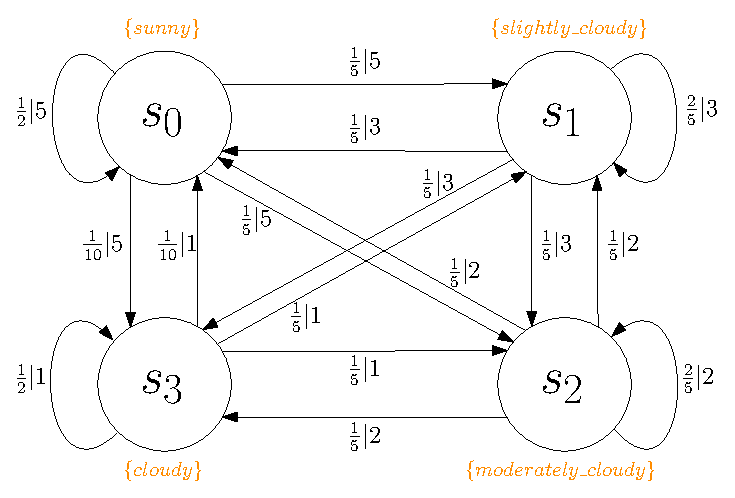
\includegraphics[width=0.5\linewidth]{resources/weather-solar-pannel}
    \captionsetup{justification=centering}
    \caption{MC modelling a daily production of energy (in $kJ$) of solar panels according to weather}
    \label{solarpanel}
  \end{figure}
  We are interested to know the probability that the weather suddenly goes from sunny to cloudy in at most three days
  (starting on a sunny day), i.e., $\mathbb{P}_{s_0}(\{s_0\} \U^{\leq 2} \{s_3\})$.
  Let $S_{=1} = \{s_3\}$ and $S_{=0} = \{ s_1, s_2 \}$, we have $S_? = \{s_0\}$. The least fixed point characterisation suggests the following iterative scheme:
  \begin{itemize}
    \item $x^{(0)} = 0$,
    \item $x^{(1)} = \Delta(s_0, s_0) \cdot x^{(0)} + \Delta(s_0, s_3) = \frac{1}{10},$ and
    \item $x^{(2)} = \Delta(s_0, s_0) \cdot x^{(1)} + \Delta(s_0, s_3) = \frac{1}{2} \cdot \frac{1}{10} + \frac{1}{10} = \frac{3}{20}$,
  \end{itemize}
  with $x^{(2)} = \mathbb{P}_{s_0}(\{s_0\} \U^{\leq 2} \{s_3\})$.
\end{example}
\begin{example}[\textit{Measuring constrained reachability event in an MC}] \label{constrained-reach-example}
Let $\mathcal{M}=(S, \Delta)$ be the MC of the figure \ref{CUTexample},
 $C = \{s_0, s_2, s_3\}$ and $T = \{s_1\}$. We are interested in the probability of the constrained reachability $C$ until $T$.
  \begin{figure}[H]
    \centering
    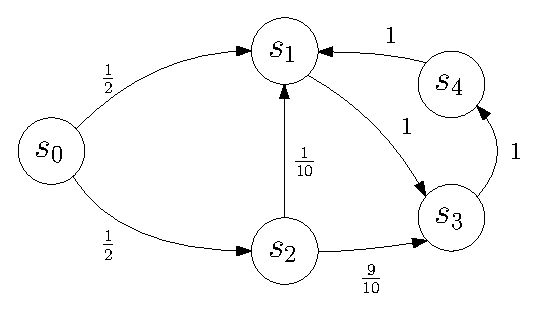
\includegraphics[width=0.4\linewidth]{resources/CUTexample}
    \captionsetup{justification=centering}
    \caption{MC $\mathcal{M}$ with state space $S = \{s_0, s_1, s_2, s_3, s_4\}$}\label{CUTexample}
  \end{figure}
  Let $S_{=1} = \{s_1\}$ and $S_{=0} = \{s \in S \; | \; \mathbb{P}_{s}(C\U T)=0\} = \{s_3, s_4\}$, we have $S_{?} = \{s_0, s_2\}$.
  The vector $(\mathbb{P}_{s}(C \U T))_{s \in S_?}$ is the unique solution of the following system:
  \begin{align*}
  	\begin{pmatrix}
      x_{s_0}\\[0.3em]
      x_{s_2}
  	\end{pmatrix} &=
    \begin{pmatrix}
      0 & \frac{1}{2} \\[0.3em]
      0 & 0
    \end{pmatrix}
    \begin{pmatrix}
      x_{s_0}\\[0.3em]
      x_{s_2}
    \end{pmatrix}
    +
    \begin{pmatrix}
      \frac{1}{2}\\[0.3em]
      \frac{1}{10}
    \end{pmatrix} \\
    \begin{pmatrix}
      x_{s_0}\\[0.3em]
      x_{s_2}
  	\end{pmatrix} &=
    \begin{pmatrix}
      \frac{1}{2} x_{s_2} \\[0.3em]
      0
    \end{pmatrix}
    +
    \begin{pmatrix}
      \frac{1}{2}\\[0.3em]
      \frac{1}{10}
    \end{pmatrix}
  \end{align*}
  So, $\mathbb{P}_{s_2}(C \U T) = x_{s_2} = \frac{1}{10}$ and $\mathbb{P}_{s_0}(C \U T) = x_{s_0} = \frac{11}{20}$.
  \\
\end{example}

With this background, we can finally introduce the following theorem.

\begin{theorem}[\textit{\textbf{Measurability of PCTL path formula events}}]
  Let $\mathcal{M}$ be an MDP with state space $S$, $s \in S$ be a state of $\mathcal{M}$ and $\phi$ be a PCTL path formula, the set $\{ \pi \in Paths(s) \; | \; \pi \models \phi \}$ is a measurable event.
\end{theorem}

\begin{proof2}
Let $Paths(s, \phi) = \{ \pi \in Paths(s) \; | \; \pi \models \phi \}$.
\begin{enumerate}
  \item If $\phi = \bigcirc \Phi$, then $Paths(s, \phi)$ agrees with the definition of $Cyl(ss')$, where $s' \models \Phi$.
  \item Else, if $\phi = \Phi_1 \U \Phi_2$, then the definition of
  $\pi \models \phi$ for any $\pi \in Paths(s)$ agrees with the definition of
  $\pi \models Sat(\Phi_1) \U Sat(\Phi_2)$.
  Thus, $Paths(s, \phi) = Sat(\Phi_1) \U Sat(\Phi_2)$.
  \item Else, if $\phi = \Phi_1 \U^{\leq n}\Phi_2$ for any $n \in \mathbb{N}$, then the definition of
  $\pi \models \phi$ for any $\pi \in Paths(s)$ agrees with the definition of
  $\pi \models Sat(\Phi_1) \U^{\leq n} Sat(\Phi_2)$.
  Thus, $Paths(s, \phi) = Sat(\Phi_1) \U^{\leq n} Sat(\Phi_2)$.
\end{enumerate}
As cylinder sets and constrained reachability events are measurable, $Paths(s, \phi)$ is measurable, for any path formula $\phi$.
\end{proof2}

\subsection{Limit behaviour}
Now, we will focus on events characterising the \textit{long-run} behaviour of Markov chains. We will address here two events : $\Box\Diamond T$ ($T$ is reached \textit{infinitely often})
and $\Diamond \Box T$ ($T$ is \textit{persistent}), for any subset of states $T \subseteq S$.
We will begin by defining these events and show that they are measurable. After that, we will introduce some graph theory notions, allowing to study the limit behaviour of Markov chains.
Studying the limit behaviour of Markov chains will allow to optimise
computations during the resolution of problems requiring linear equations systems or linear programs. Moreover, it will allow fast computations to determine probabilities of \textit{infinitely often} and \textit{persistent} events.

\begin{definition}[\textbf{Infinitely often event}]
  Let $\mathcal{M}=(S, \Delta, w, AP, L)$ be an MC, $T \subseteq S$, be a subset of states of $\mathcal{M}$, and
  $s \in S$ be a state of $\mathcal{M}$ from which events start. For any path $\pi = s_0 s_1 s_2 \dots \in Paths(s)$,
encountering \textit{infinitely often} $T$ actually means that, for all index $n \in \mathbb{N}$ (and thus, for any step $s_n$ of $\pi$), there exists an index $m \geq n$ such that $s_m \in T$. Then, let
  \begin{align*}
    Paths_{fin}^{m,\, T}(s) &= \{ s_0\dots s_m \in Paths_{fin}(s) \; | \; s_m \in T \}, \text{ and} \\
    Cyl^{m,\, T}(s) &= \bigcup_{s_0 \dots s_m \in Paths_{fin}^{m, \, T}(s)} Cyl(s_0\dots s_m)
  \end{align*}
  for any number of steps $m \in \mathbb{N}$. The infinitely often event for $T$ is defined as follows:
  \[
    \Box \Diamond T = \bigcap_{n \in \mathbb{N}} \bigcup_{m \geq n} Cyl^{m, \, T}(s).
  \]
  Since $\Box \Diamond T$ is formed by intersections of unions of cylinder sets, this event is measurable, and $\mathbb{P}_s(\Box\Diamond T)$ actually denotes the probability measure of this event, starting from the state $s \in S$.
\end{definition}

\begin{definition}[\textbf{Persistence event}]
  Let $\mathcal{M}=(S, \Delta, w, AP, L)$ be an MC, $T \subseteq S$, be a subset of states of $\mathcal{M}$, and
  $s \in S$ be a state of $\mathcal{M}$ from which events start. For any path $\pi = s_0 s_1 s_2 \dots \in Paths(s)$,
 $T$ is \textit{persistent} actually means there exists an index $n \in \mathbb{N}$ such that, for all $i\geq n$, $s_i \in T$. The persistence event for $T$ is defined as follows:
 \[
  \Diamond \Box T = \overline{\Box \Diamond (S \setminus T)}.
 \]
 Since $\Box \Diamond (S \setminus T)$ is measurable, $\Diamond \Box T$ is measurable, with \[\mathbb{P}_s(\Diamond \Box T) = 1 - \mathbb{P}_s(\Box \Diamond (S \setminus T)).\]
\end{definition}
We will now provide a way to compute the probability of these events with purely graph theory algorithms. To do that, we need to introduce some graph concepts.

\begin{definition}[\textbf{Bottom strongly connected components}]
Let $\mathcal{M}=(S, \Delta, w, AP, L)$ be an MC and $T \subseteq S$ be a subset of states of $\mathcal{M}$.
\begin{itemize}
  \item $T$ is \textit{strongly connected} if for any $s, s' \in T$, $s$ is connected to $s'$ in the underlying graph of $\mathcal{M}$, i.e., if there exists a finite path $s_0 \dots s_k \in Paths_{fin}(s)$ from $s$ to $s'$ in $\mathcal{M}$ such that $s_k = s'$.
  \item $T$ is a \textit{strongly connected component} (i.e., an \textbf{SCC}) of $\mathcal{M}$ iff $T$ is strongly connected and no proper superset of $T$ is strongly connected, i.e.,
  \[ T \text{ is strongly connected } \, \wedge \,
  \neg(\exists T', \; T' \text{ is strongly connected } \wedge \;
    T \subseteq T'). \]
  \item $T$ is a \textit{bottom strongly connected component} (i.e., a \textbf{BSCC}) of $\mathcal{M}$ iff
  $T$ is a SCC and no state outside $T$ can be reached, i.e.,
  \[
  T \text{ is an SCC} \; \wedge \; \forall s \in T, \,\Delta(s, T) = 1.
  \]
\end{itemize}
\end{definition}

SCCs and BSCCs of any Markov chain can be computed with
purely graph theory algorithms (e.g., with depth-first search algorithms based).

\begin{example}[\textit{Difference between SCCs and BSCCs}]
Let $\mathcal{M}=(S, \Delta)$ be the MC of the figure \ref{bsccex}. We have that the subset $T = \{s_1, s_2, s_3\} \subseteq S$ is an SCC because $T$ is the largest subset containing the state $s_1$ such that all states are connected to each other.
However, $T$ is not a BSCC because the state $s_3 \in T$ is connected by an edge in the underlying graph of $\mathcal{M}$ (we have $\Delta(s_3, s_4) > 0$), and $s_4$ is not connected to $T$.
Furthermore, the subset $B = \{s_5, s_6, s_7, s_8\} \subseteq S$ is a BSCC. Indeed, $B$ is the largest subset of $S$ containing $s_5$ such that all states are connected to each other. Moreover, each state $s \in B$ verify the following assertion:
$\Delta(s, B)=1$.
  \begin{figure}[h!]
    \centering
    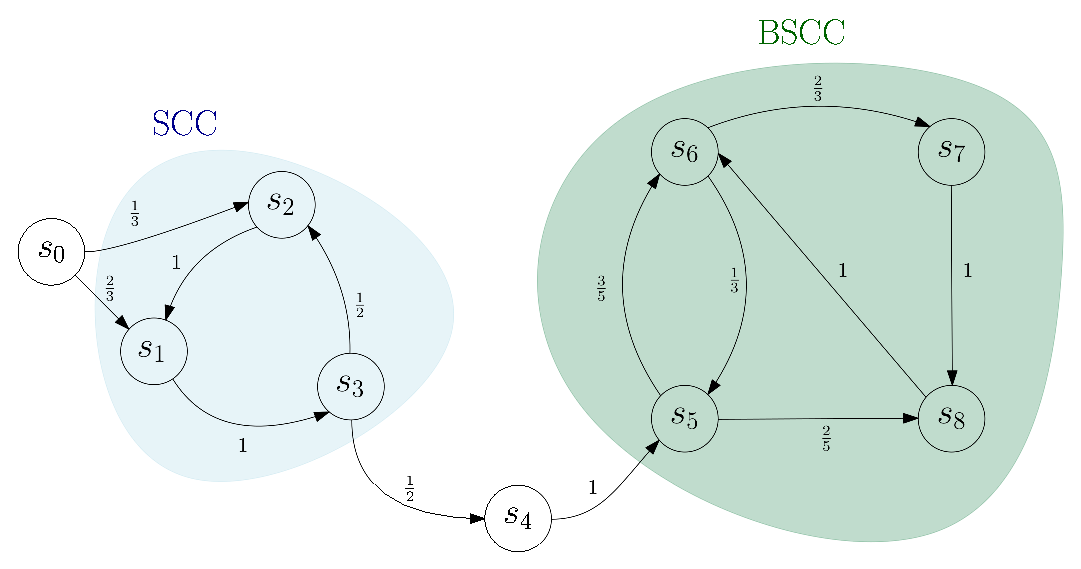
\includegraphics[width=0.7\linewidth]{resources/BSCC}
    \captionsetup{justification=centering}
    \caption{Markov chain $\mathcal{M}$ with state space composed by nine states, containing two SCCs and one BSCC}\label{bsccex}
  \end{figure}
\end{example}

\begin{theorem}[\textit{\textbf{Limit behaviour of Markov chains}}]\label{MCbehav}
Let $\mathcal{M}$ be an MC with state space $S$ and $s \in S$
be a state of $\mathcal{M}$ from which events start,
\[
  \mathbb{P}_s(\{\pi \in Paths(s) \; | \; inf(\pi) \text{ is a BSCC of }\mathcal{M}\}) = 1,
\]
where the $inf(\pi)$ denotes the set of states encountered infinitely often along $\pi = s_0 s_1 s_2 \dots \in Paths(s)$, i.e., $inf(\pi) = \{ s \in S \; | \; \forall n \in \mathbb{N},\, \exists m \geq n,\, s_m = s\}$.
\end{theorem}
A consequence of the theorem \ref{MCbehav} is that, starting from any state of a MC, the system ends up in a BSCC with probability one, and all states of this BSCC are visited infinitely often.

\begin{corollary}[\textbf{\textit{Quantitative repeated reachability}}]
  Let $\mathcal{M}$ be a finite MC with state space $S$, $T \subseteq S$ be a subset of states of $\mathcal{M}$, and $s \in S$ be a state of $\mathcal{M}$.
  Then, we can compute the probability to encounter infinitely often $T$ as follows:
  \[
    \mathbb{P}_s(\Box \Diamond T) = \mathbb{P}_s(\Diamond U),
  \]
  where $U$ is the union of all BSCCs $B$ of $\mathcal{M}$ such that $B \cap T \neq \emptyset$. Furthermore, we can compute the probability that $T$ is persistent as follows:
  \[
    \mathbb{P}_s(\Diamond \Box T) = \mathbb{P}_s(\Diamond U),
  \]
  where $U$ is the union of all BSCCs $B$ of $\mathcal{M}$ such that $B \subseteq T$.
\end{corollary}

\begin{proof2}
Let $BSCC(\mathcal{M})$ denotes the set of BSCCs of $\mathcal{M}$.
\begin{enumerate}
\item
Let $B \in BSCC(\mathcal{M})$ be a BSCC of $\mathcal{M}$.
In particular, let assume there exists a state $t \in T$ such that $t \in B$, then $\mathbb{P}_s(\Diamond B) = \mathbb{P}_s(\{ \pi \in Paths(s) \; | \; t \in inf(\pi) \; \wedge \; inf(\pi) = B \})$. Following the definition of BSCCs, we have that $B$ is the largest subset containing $t$ such that all states of $B$ are connected to each other and such that $\forall s' \in B, \, \Delta(s', B)=1$. Then, $B$ is the only BSCC containing $t$. So,
$\mathbb{P}_s(\Diamond B) = \mathbb{P}_s(\{ \pi \in Paths(s) \; | \; t \in inf(\pi)\}) = \mathbb{P}_s(\Box \Diamond \{t\})$,
by definition of $inf(\pi)$ and $\Box\Diamond \{t\}$.
\label{B1}
%\item Furthermore, let $t \in T$, it stills to show that if $\mathbb{P}_s(\Box \Diamond \{t\}) > 0$, then we always have that there exists a BSCC $B$ such that $\mathbb{P}_s(\Diamond B)>0$, $t \in B$. By contraposition, let assume that for all BSCC $B$ such that $\mathbb{P}_s(\Diamond B) > 0$, $t \centernot\in B$.
\item
Furthermore, let assume that for all BSCC $B$, $t \notin B$. As we have \[\mathbb{P}_s(\{\pi \in Paths(s)\; | \; t \notin inf(\pi), \, inf(\pi) \in BSCC(\mathcal{M})\}) = 1,\]
we obviously have $\mathbb{P}_s(\{\pi \in Paths(s)\; | \; t \in inf(\pi)\}) = 0$, i.e., $t$ is never visited infinitely often with a positive probability, and $\mathbb{P}_s(\Box\Diamond \{t\}) = 0$.
\label{B2}
\end{enumerate}
%A consequence of the theorem \ref{MCbehav} is that
%$\mathbb{P}_s(\Diamond \bigcup_{B \in BSCC(\mathcal{M})} B)
%= 1$. Then, there exists $B \in BSCC(\mathcal{M})$ such
%that $\mathbb{P}_s(\Diamond B) > 0$. If $t \in B$, then we
%have $\mathbb{P}_s(\Box\Diamond\{t\})>0$.
We can generalise \ref{B1} and \ref{B2} for all states in the set $T$:
\[\mathbb{P}_s(\Box \Diamond T) = \mathbb{P}_s(\Diamond \bigcup_{B \in BSCC(\mathcal{M}) \; | \; \exists t \in T, \, t \in B } B)\]
The second assertion can be shown in a similar way.
%\vspace{-0.1\linewidth}
\end{proof2}\\

Now, we will come back on a problem addressed previously in the remark \ref{remarkS0S1}. Indeed, following an MC $\mathcal{M}$ with state space $S$ and two subsets $C, T \subseteq S$, we have presented a graph theory based solution to compute the largest subset $S_{=0}$, i.e., $\{s \in S \; | \; \mathbb{P}_s(C \U T) = 0\}$, but we have not yet presented a solution to compute the largest subset $S_{=1}$, i.e., $\{s \in S \; | \; \mathbb{P}_s(C \U T) = 1\}$.
We will see that qualitative properties can be verified thanks to the notion of BSCC.

\begin{notation}[\textit{Absorbing state}]
  Let $\mathcal{M}=(S, \Delta, w, AP, L)$ be an MC and $s \in S$ be a state of $\mathcal{M}$. We say that $s$ is absorbing iff $\Delta(s, s') = 1$.
\end{notation}

\begin{theorem}[\textbf{\textit{Almost sure reachability}}]\label{asr}
  Let $\mathcal{M}$ be a finite MC with state space $S$, $s \in S$ be a state of $\mathcal{M}$ from which events start, $T \subseteq S$ be a set of absorbing states, and the two following successors and predecessors sets:
\begin{align*}
  Succ^*(s) &= \{ s' \in S \; | \; \exists \pi = s_0s_1s_2\dots \in Paths(s) \;\; \exists k \in \mathbb{N}_0, \, s_k = s' \}, \\
  Pred^*(T) &= \{ s' \in S \; | \; \exists \pi = s_0s_1s_2\dots \in Paths(s')\; \exists k \in \mathbb{N}_0, \, s_{k} \in T \,\}.
\end{align*}
   Then , the following statements are equivalent:
  \begin{enumerate}[(a)]
    \item $\mathbb{P}_s(\Diamond T)= 1$. \label{succ1}
    \item $Succ^*(s') \cap T \neq \emptyset, \; \forall s' \in Succ^*(s)$.\label{succ2}
    \item $s \in S \setminus Pred^*(S \setminus Pred^*(T))$. \label{succ3}
  \end{enumerate}
  In particular, \[
  \{s \in S \; | \; \mathbb{P}_s(\Diamond T) = 1\} =
  S \setminus Pred^*(S \setminus Pred^*(T))
  \]
  \begin{figure}[h]
  \centering
  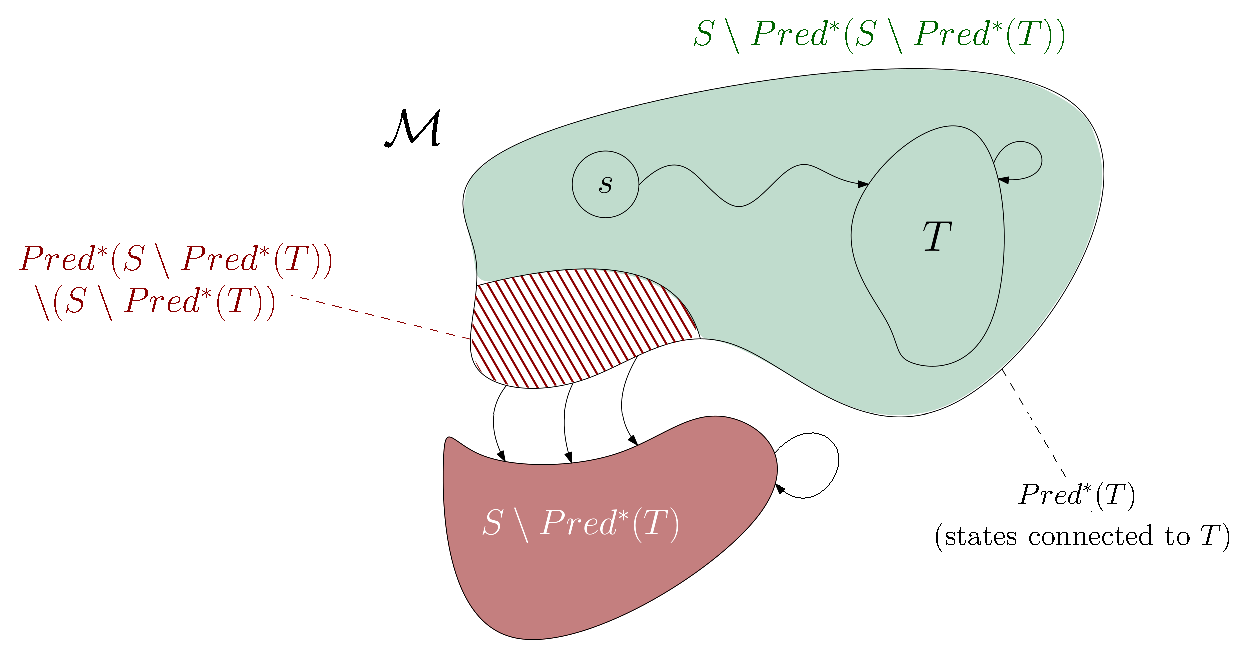
\includegraphics[width=0.8\linewidth]{resources/S1BSCC}
  \caption{Intuitive representation of the subset $S \setminus Pred^*(S \setminus Pred^*(T))$}\label{spred}
  \end{figure}
\end{theorem}
\begin{proof2}\cite{PMC}
We can easily derivate from the definitions of the sets $Succ^*$ and $Pred^*$ that \ref{succ2} and \ref{succ3} are equivalent. \\
($\neg\ref{succ2}\implies\neg\ref{succ1}$). Let $s' \in Succ^*(s)$ such that $Succ^*(s') \cap T = \emptyset$ Following the figure \ref{spred}, we have that $s$ is in the subset represented by a red tiling pattern or $s$ is in the red subset and we have that $s'$ is in the red subset. Thus, $s'$ is a successor of $s$ from which $T$ can not be reached. Then, we have $\mathbb{P}_s(\Diamond T) \leq 1 - \mathbb{P}_s(\Diamond \{s'\}) < 1$.
%Furthermore, referring the figure
%\ref{spred}, we have that $1 - \mathbb{P}_s(\Diamond T) = \mathbb{P}_s(\Diamond (S \setminus Pred^*(T)))$.\\
($\ref{succ2} \implies \ref{succ1}$). Let assume that $Succ^*(s') \cap T \neq \emptyset$, for any successor $s'$ of $s$. By the theorem \ref{MCbehav}, we reach a BSCC from $s$ with a probability one. Since each state in $t \in T$ is absorbing, each BSCC $B$ of $\mathcal{M}$ consists in $B = \{t\}$ or it satisfies $T \cap B = \emptyset$. We will show that the latter case can not occur from $s$.
Consider $T \cap B = \emptyset$ for BSCC $B$.
As $B$ is a BSCC, $Succ^*(u)\cap T = \emptyset$, for each $u \in B$.
However, as $T$ is reachable for any $s' \in Succ^*(s)$, there is no BSCC with $T \cap B = \emptyset$ that is reachable from $s$. So, we almost surely have a state in $T$ that will be reached from the state $s$.
\end{proof2}
\\

The theorem \ref{asr} allows to compute the largest subset $S_{=1} = \{s \in S \; | \; \mathbb{P}_s(\Diamond T) = 1 \}$ for any finite MC with state space $S$ and for any $T \subseteq S$ as follows:
%Indeed, we begin by make all states in $T$ absorbing. This allows to apply the theorem \ref{asr}.
%Then, we can compute all states connected
\begin{algorithm}[H]
\caption{Almost sure reachability}\label{almost-sure-algo}
\begin{algorithmic}[1]
  \REQUIRE a finite Markov chain $\mathcal{M}$ with state space $S$, a transition function $\Delta$, and a set of target states $T \subseteq S$.
  \ENSURE the set $\{ s \in S \; | \; \mathbb{P}_s(\Diamond T) = 1\}$.
  \item[]
  \STATE $\Delta_T \leftarrow \lambda (s, s'):\, \begin{cases}
    1 &\text{if } s = s' \text{ and } s \in T\\
    \Delta(s, s') &\text{else}
  \end{cases}$
  \STATE $\mathcal{M}_T \leftarrow (S, \Delta_T)$
  \COMMENT{make all states of $T$ absorbing, yielding a new MC $\mathcal{M}_T$}
  \STATE $Pre^*(T) \leftarrow \mathsf{backward\_search}(G^{\mathcal{M}_T}, T)$
  \COMMENT{compute the set of states connected to $T$}
  \STATE $Pre^*(S \setminus Pre^*(T)) \leftarrow \mathsf{backward\_search}(G^{\mathcal{M}_T}, S \setminus Pre^*(T))$
  \RETURN $S \setminus Pre^*(S \setminus Pre^*(T))$
\end{algorithmic}
\end{algorithm}
\noindent where the notation $\lambda x:y$ is a lambda calculus based notation that gives the lambda calculus expression $\lambda x.y \equiv x \mapsto y$, $G^\mathcal{M}$ denotes the underlying graph of $\mathcal{M}$ and the $\mathsf{backward\_search}$ algorithm
, for inputs $G^{\mathcal{M}_T}$ and $T$, explores $G^{\mathcal{M}_T}$ from the set $T$: it starts by marking all states of $T$, and then iteratively marks all unmarked predecessors of marked states (\textit{backward breadth-first search}). All marked states are thus connected to $T$. An alternative recursive version of this algorithm exists (\textit{backward depth-first search}).
The time complexity of this algorithm is in $\mathcal{O}(|\mathcal{M}_T|)$.

\begin{corollary}[\textbf{\textit{Qualitative constrained reachability}}] Let $\mathcal{M}$ be a finite MC with state space $S$ and $C, T \subseteq S$, the sets
\[
  S_{=0} = \{ s \in S \; | \; \mathbb{P}_s (C \U T) = 0 \} \text{ and } S_{=1} = \{ s \in S \; | \; \mathbb{P}_s (C \U T ) = 1 \}
  \]
  can be computed in time $\mathcal{O}(|\mathcal{M}|)$.
\end{corollary}
\begin{proof2}\cite{PMC}
\begin{enumerate}
  \item We can determine $S_{=0}=\{s \in S \; | \; \mathbb{P}_s(C \U T)=0\}$ by computing the complement of the set $\{s \in S \; | \; \exists \pi \in Paths(\pi), \, \pi \models C \U T \}$ (cf. lemma \ref{S0graph}).
  \item A linear-time algorithm for the computation of $S_{=1}=\{ s\in S \; | \; \mathbb{P}_s(C \U T) = 1 \}$ can be solved by a reduction to the reachability problem to $T$ in a slightly modified MC. The idea is the following: we make all states of $T$ absorbing (to take advantage of the theorem \ref{asr}) and do the same for all states in $S \setminus (C \cup T)$.
  The probability transition function of this modified MC $\mathcal{M}'$ is
  defined as follows:
  \[
    \Delta'(s, s') = \begin{cases}
      1 & \text{if } s=s' \text{ and } s'\in T \cup S \setminus(C \cup T),\\
      0 & \text{if } s \neq s' \text{ and } s \in T \cup S \setminus (C \cup T),\, \text{and}\\
      \Delta(s, s') & \text{otherwise}.
    \end{cases}
  \]
  Thus, we have:
  \begin{itemize}
    \item $\mathbb{P}_s^\mathcal{M}(C \U T) = \mathbb{P}_s^\mathcal{M'}(\Diamond T)$ for all states $s \in C \setminus T$,
    \item $\mathbb{P}_s^\mathcal{M}(C \U T) = \mathbb{P}_s^{\mathcal{M}'}(\Diamond T) = 1$
    for all states $s \in T$, and
    \item $\mathbb{P}_s^\mathcal{M}(C \U T)= \mathbb{P}_s^{\mathcal{M}'}(\Diamond T) = 0$ for all states $s \in S \setminus (C \cup T)$.
  \end{itemize}
  Doing this reduction, we can now apply the lemma \ref{S0graph} on $\mathcal{M}'$ to compute the largest set $S_{=0}$. Since $\Diamond T = S \U T$, we have $S_{=0}= S \setminus Pred^*(T)$. Then, we can apply the theorem  \ref{asr} to compute the largest set $S_{=1}$ with the algorithm \ref{almost-sure-algo}.
\end{enumerate}
\end{proof2}\\

Thus, check if each temporal events presented in this section holds with a probability one or zero can be done through simple graph theory algorithms in $\mathcal{O}(|\mathcal{M}|)$, without referring to probabilities of transitions.

\section{PCTL model checking}
\begin{definition}[\bfseries PCTL model checking]
Let $\mathcal{M}$ be an MC with state space $S$, $s \in S$ be a state of $\mathcal{M}$, and $\Phi$ be a PCTL state formula. The model checking problem for $\mathcal{M}$, $s$ and $\Phi$ consists of deciding if $s \models \Phi$, i.e., if $s \in Sat(\Phi)$.
\end{definition}
Following an MC $\mathcal{M}$, a state $s$ of this MC and a state formula $\Phi$, determine if $s \models \Phi$ can be done through a bottom-up traversal of the \textit{parse tree} of $\Phi$.
Indeed, according to the PCTL syntax, we recursively decompose $\Phi$ following its sub-formulae. Moreover, each sub-formula of $\Phi$ is actually represented by a node of this tree. For each PCTL state formula $\Phi$, we compute its satisfaction set from the node representing the formula, according to each satisfaction set computed from each of its child and the characterisation of $Sat(\Phi)$.
\begin{property}[Characterisation of Sat]
Let $\mathcal{M} = (S, \Delta, w, AP, L)$ be an MC, $\Phi, \Psi$ be PCTL state formulae over $AP$, and $\phi$ be a  PCTL path formula over $AP$. The satisfaction set $Sat$ is characterised as follows:
\begin{flalign*}
  Sat(true) &= S,\\
  Sat(a) &= \{s \in S \; | \; a \in L(s)\} \text{ for } a \in AP,\\
  Sat(\Phi) \, \wedge \, Sat(\Psi) &= Sat(\Phi) \cap Sat(\Psi),\\
  Sat(\neg \Phi) &= S \setminus Sat(\Phi), \text{ and} \\
  Sat(\mathcal{P}_J(\phi)) &= \{ s \in S \; | \; \mathbb{P}_s (Paths(s, \phi)) \in J \} \text{ for } J \subseteq [0, 1],
\end{flalign*}
where $Paths(s, \phi) = \{ \pi \in Paths(s) \; | \; \pi \models \phi \}$.
$\mathcal{P}_J(\phi)$ is computed according to the formula $\phi$ as follows:
let $s \in S$ be a state of $\mathcal{M}$,
\begin{flalign*}
  \mathbb{P}_s(Paths(s,\, \bigcirc \Phi)) &= \sum_{s' \in Sat(\Phi)} \Delta(s, s'), \\
  \mathbb{P}_s(Paths(s,\, \Phi \U \Psi)) &= \mathbb{P}_s(Sat(\Phi) \U Sat(\Psi)), \text{ and}\\
  \mathbb{P}_s(Paths(s, \, \Phi \U^{\leq n} \Psi)) &=
    \mathbb{P}_s(Sat(\Phi) \U^{\leq n} Sat(\Psi)). \tag{cf. section \ref{tempevent}}
\end{flalign*}
Additionally, we can optimise the computation of the satisfiability sets of the following formulae:
\begin{align*}
  Sat(\mathcal{P}_J(\Diamond \mathcal{P}_{=1} (\Box \mathcal{P}_{=1}(\Diamond a)))) &=
\{ s \in S \; | \; \mathbb{P}_s (\Box \Diamond Sat(a)) \in J \}, \tag{\textit{\small infinitely often}} \\
Sat(\mathcal{P}_J(\Diamond \mathcal{P}_{=1}(\Box a))) &= \{ s \in S \; | \; \mathbb{P}_s(\Diamond \Box Sat(a)) \in J\}, \tag{\textit{persistence}}
\end{align*}
for $J \subseteq [0, 1]$ and $a \in AP$.
\end{property}

\begin{example}[\textit{PCTL model checking of an MC via its parse tree}]
  Let $\mathcal{M}=(S, \Delta, w, AP, L)$ be the MC of the figure \ref{CUTexample2} and the state formula $\Phi = c \vee \mathcal{P}_{\geq \frac{1}{2}}(a \U (b \wedge c))$.
  \begin{figure}[h!]
  \begin{minipage}{0.4\linewidth}
    \centering
    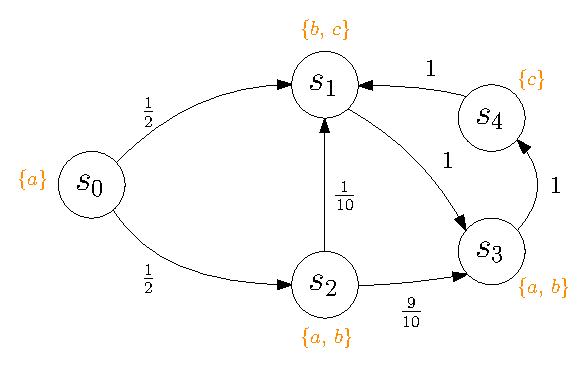
\includegraphics[width=\linewidth]{resources/CUTexample2}
    \captionsetup{justification=centering}
    \captionof{figure}{MC $\mathcal{M}$ with state space $S = \{s_0, s_1, s_2, s_3, s_4\}$ and atomic propositions of the set $AP = \{a, b, c\}$}
    \label{CUTexample2}
  \end{minipage}
    $ \quad $
  \begin{minipage}{0.6\linewidth}
    \centering
    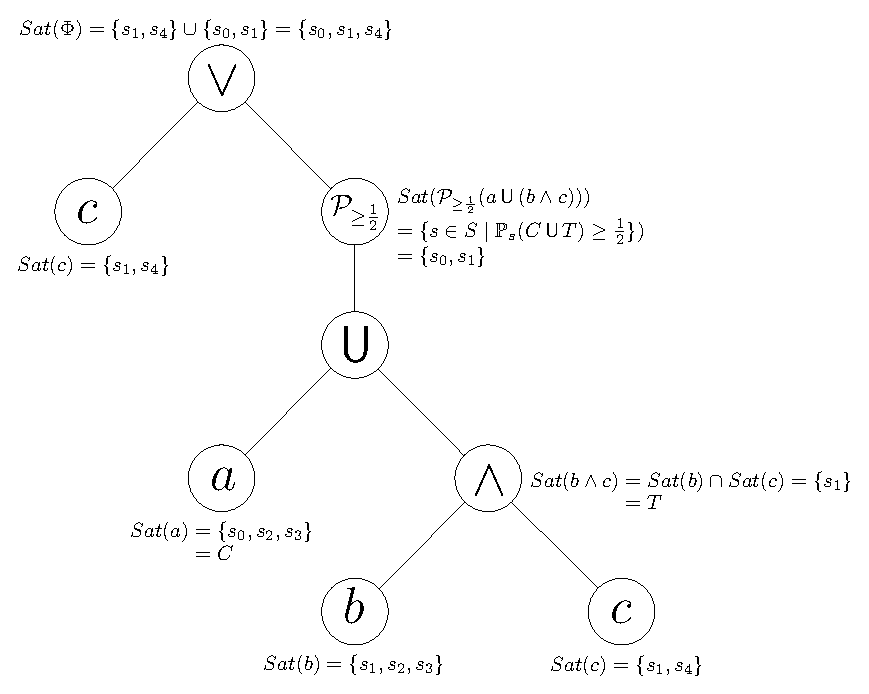
\includegraphics[width=\linewidth]{resources/parse-tree}
    \captionsetup{justification=centering}
    \captionof{figure}{Parse tree of $\mathcal{M}$ for $\Phi$}
    \label{parse-tree-example}
  \end{minipage}
  \end{figure}
  We are interested to know if $s_0 \models \Phi$. To do that, we build the parse tree of $\Phi$.
  This one is given in the figure \ref{parse-tree-example}. We can compute $Sat(\Phi)$ through a bottom up traversal of this tree: we begin at the leaves of the tree, i.e., by computing $Sat(a)$, $Sat(b)$, and $Sat(c)$. Then, we compute $Sat(b \wedge c)$, that equals $Sat(b)\cap Sat(c)$, according to the characterisation of the satisfaction set.
  After that, we compute
  $Sat(\mathcal{P}_{\geq \frac{1}{2}}(a \U (b \wedge c)))$ by computing $\{ s \in S \; | \; \mathbb{P}_s(Sat(a) \U Sat(b \wedge c)) \geq \frac{1}{2}\} = \{ s \in S \; | \; \mathbb{P}_s(\{s_0, s_2, s_3\} \U \{s_1\}) \geq \frac{1}{2}\}$.
  We actually have already computed these probabilities (cf. example \ref{constrained-reach-example}).
  So, this set equals $\{ s_0, s_1 \}$.
  Finally, since we have already computed $Sat(c)$ and $Sat(\mathcal{P}_{\geq \frac{1}{2}}(a \U (b \wedge c)))$, we can compute $Sat(\Phi) = \{s_1, s_4\} \cup \{s_0, s_1\} = \{s_0, s_1, s_4\}$.
  As $s_0 \in Sat(\Phi)$, then $s_0 \models \Phi$.
\end{example}

\section{PCTL for Markov decision processes}
The PCTL syntax for MDPs is exactly the same as for MCs with the exception of the probabilistic operator $\mathcal{P}_J(.)$ due to the nondeterminism of MDPs:
we can not verify probabilistic properties without referring to the notion of strategy.
Then, we replace this operator with $\mathcal{P}^{\max}_J(.)$, referring to the strategy offering the maximum probability of satisfying a given property.
Thus, the formula $\mathcal{P}^{\max}_J(\phi)$ asserts \[\mathbb{P}^{\max}_s(\{\pi \in Paths(s) \; | \; \pi \models \phi \}) \in J .\]
\textit{Note: remind that $\mathbb{P}_s^{\max}(E)$ refers to the probability measure defined on the MC induced by the strategy maximising the probability of the event $E$ in this MC, i.e., $\max_{\sigma} \mathbb{P}_s^\sigma(E)$.}

\begin{definition}[\textbf{Syntax of PCTL for MDPs}]
Let $AP$ be a set of atomic propositions,
\begin{itemize}
  \item PCTL \textit{state formulae} are formed according the following grammar:
  \[
    \Phi ::= true \;\; | \;\; a \;\; | \;\; \Phi_1 \wedge \Phi_2 \;\; | \;\; \neg \Phi \;\; | \;\; \mathcal{P}^{\max}_J(\phi)
  \]
  where $a \in AP$ is an atomic proposition, $J \subseteq [0, 1]$ gives probability bounds and $\phi$ is a path formula.
  \item PCTL \textit{path formulae} are formed according
  to the same grammar than for MCs.
\end{itemize}
\end{definition}
\begin{definition}[\textbf{Semantic of PCTL for MDPs}]
  Let $\mathcal{M} = (S, A, \Delta, AP, L)$ be an MDP and $s \in S$, be a state of $\mathcal{M}$,
  \begin{flalign*}
  \intertext{$s \models \Phi$ iff the state formula $\Phi$ holds in the state $s$, i.e.,}
    &\bigcdot\; s \models true, &&&\\
    &\bigcdot\; s \models a &\text{ iff }& a \text{ is a label of $s$, i.e., } a \in L(s),&\\
    &\bigcdot\; s \models \Phi_1 \wedge \Phi_2&\text{ iff }& s \models \Phi_1 \text{ and } s \models \Phi_2,&\\
    &\bigcdot\; s \models \neg \Phi &\text{ iff }& s \not\models \Phi, &\\
    &\bigcdot\; s \models \mathcal{P}^{\max}_J(\phi) &\text{ iff }& \mathbb{P}^{\max}_s(\{ \pi \in Paths(s) \; | \; \pi \models \phi \}) \in J.&
  \intertext{$\pi \models \phi$ iff the $\pi$ satisfies $\phi$ in the induced MC.}
  \end{flalign*}
\end{definition}
In the first chapter, we have addressed a way to compute the strategy $\sigma$ to resolve the SR problem, i.e., compute the strategy $\sigma$ following an MDP $\mathcal{M}$ with state space $S$, a state $s \in S$, and a subset of target states $T$, such that $\mathbb{P}_s^\sigma(\Diamond T) = \mathbb{P}^{\max}_s(\Diamond T)$.
We have seen that this can be done in polynomial time in the size of $\mathcal{M}$, through a linear program (cf. theorem \ref{thm-sr} and appendix \ref{app-sr}).
We can generalise this computation of optimal strategy for the constrained reachability events. To this purpose, we need to address the equation system from which the linear program used to compute this strategy is derived (cf. appendix \ref{app-sr}).

\begin{theorem}[\textbf{Equation system for max reachability probabilities}]
  Let $\mathcal{M}$ be a finite MDP with state space $S$ and with a probability transition function $\Delta$, $s \in S$ be a state of $\mathcal{M}$ and $T \subseteq S$ be a subset of target states. The vector $(x_s)_{s \in S}$ with $x_s = \mathbb{P}_s^{\max}(\Diamond T)$ yields the unique solution of the following equation system: let the subset $S_{=1} \subseteq S$ be a subset of states such that $T \subseteq S_{=1} \subseteq \{s \in S \; | \; \mathbb{P}^{\max}_s(\Diamond T) = 1 \}$,
  \begin{itemize}
    \item if $s \in S_{=1}$, then $x_s=1$,
    \item else if $s$ is not connected to $T$ in the underlying graph of $\mathcal{M}$, then $x_s=0$,
    \item else,
    \[ x_s = \max_{\alpha \in A(s)} \sum_{s' \in Succ(s, \alpha)} \Delta(s, \alpha, s') \cdot x_{s'}. \]
  \end{itemize}
\end{theorem}
This theorem suggests an iterative approximation technique, called \textit{value iteration}, to compute the values $x_s=\mathbb{P}^{\max}_s(\Diamond T)$. First, we fix the values of $x_s^{(n)} = x_s$, for all $n \in \mathbb{N}$, according to the two first conditions of the equation system by a backward reachability analysis of the underlying graph of $\mathcal{M}$. For other states $s$, we have
\[x_s = \lim_{n \rightarrow \infty} x_s^{(n)}\]
where
\[x_s^{(0)} = 0 \quad \text{and} \quad x_s^{(n+1)} = \max_{\alpha \in A(s)} \sum_{s' \in Succ(s, \alpha)} \Delta(s, \alpha, s') \cdot x_{s'}^{(n)}. \]
This yields $x_s^{(n)} \leq x_s^{(n+1)}$ for any $n \in \mathbb{N}$, and the values of $\mathbb{P}^{\max}_s(\Diamond T)$ can be approximated by iteratively computing vectors $x_s^{(n+1)}$
with vectors $x_s^{(n)}$ for all states $s \in S$ until $\max_{s \in S} |x_s^{(n+1)} - x_s{(n)}| < \varepsilon$ for a small threshold value $\varepsilon > 0$.
\begin{theorem}[\textbf{Value iteration for step-bounded reachability}]
  Let $\mathcal{M}$ be a finite MDP with state space $S$ and with a probability transition function $\Delta$, and a subset of target states $T \subseteq S$. The value iteration approach can be used to compute the maximal probabilities for the event $\Diamond^{\leq n}T$.
  Indeed, the vector $(x_s)^{(n)}_{s \in S}$ with $x_s^{(n)} = \mathbb{P}^{\max}_s(\Diamond^{\leq n} T)$ yields the unique solution of the following equation system:
  \begin{itemize}
    \item if $s \in T$, then $x_s^{(n)}=1$ for all $n \in \mathbb{N}$,
    \item else if $s$ is not connected to $T$ in the underlying graph of $\mathcal{M}$, then $x_s^{(n)}=0$
    for all $n \in \mathbb{N}$,
    \item else, $x_s^{(0)} = 0$ and
    \[ x_s^{(n+1)} = \max_{\alpha \in A(s)} \sum_{s' \in Succ(s, \alpha)} \Delta(s, \alpha, s') \cdot x_{s'}^{(n)}. \]
  \end{itemize}
  According to this equation system, we can build a finite memory strategy $\sigma = (Q, \sigma_\alpha, \delta, \delta_0)$ such that $\mathbb{P}^\sigma_s(\Diamond^{\leq n} T) = \mathbb{P}^{\max}_s(\Diamond^{\leq n} T)$ for $s \in S$ and $n \in \mathbb{N}$:
  assume that modes of $Q$ range from $0$ to $n$ such that $\delta_0(s) = m_0$ and $\delta(m_i, s) = m_{\min\{i+1, n\}}$ for all $s \in S$ and $i \in \{0, \dots, n\}$. Then, we define $\sigma_\alpha$ as follows:
  \[
    \sigma_\alpha(m_i, s) =
    \begin{cases}
      \alpha \; \text{ such that } \alpha \in A(s) &\text{if }i=0,\\
      \arg \max_{\alpha \in A(s)} \sum_{s' \in Succ(s, \alpha)} \Delta(s, \alpha, s') \cdot x_{s'}^{(i-1)}
      & \text{else.}
    \end{cases}
  \]
  Intuitively, $\sigma$ is initialised in mode $m_0$, and when the strategy is in mode $m_i$, $i \in \{1, \dots, n-1\}$,
  it chooses the action that maximises $\sum_{s' \in Succ(s, \alpha)} \Delta(s, \alpha, s') \cdot x_{s'}^{(i-1)}$ and then changes its mode $m_i$ to the next mode $m_{i+1}$. When the strategy is in mode $m_n$, it stays inside it forever.
\end{theorem}
As for MCs, we can compute constrained reachability events $C \U T$ or $C \U^{\leq n} T$ by reduction to the reachability to $T$ as follows:
we make all states of $s \in S \setminus (C \cup T)$ absorbing i.e., we replace all the enabled actions of $A(s)$
by an unique action $\alpha_s$ such that $\Delta(s, \alpha_s, s) = 1$.
Then, we compute $\mathbb{P}^{\max}_s(\Diamond T)$ in this modified MDP to get the linked strategy.


\bibliographystyle{plain}
\bibliography{bib}

\chapter*{Appendix}
\addcontentsline{toc}{chapter}{Appendix}
\markboth{Appendix}{Appendix}
\stepcounter{chapter}

\section{Linear equations systems}
\subsection{Reachability in a MC}
Let $\mathcal{M} = (S, \Delta, w, AP, L)$ be a MC, $s \in S$ be a state of $\mathcal{M}$ and $T \subseteq S$ be a set of target states in $\mathcal{M}$.
We can compute the probability to reach $T$ from $s$ :
let $(x_s)_{s \in S}$ be a vector of probabilities,
\begin{itemize}
	\item if $s$ is not connected to $T$ in the underlying graph of $\mathcal{M}$, then we have $x_s = 0$
	\item else, if $s \in T$, then we obviously have $x_s = 1$
	\item else, for all $s \in S \setminus T$  such that $s$ is connected to $T$ in the underlying graph of $\mathcal{M}$,
		\[
      x_s = \underbrace{\sum_{s' \in S \setminus T} \Delta(s, s') \cdot x_{s'}}_{\text{reach $T$ via $s' \in S \setminus T$}} + \underbrace{\sum_{t \in T} \Delta(s, t)}_{\text{reach $T$ in one transition}}
    \]
\end{itemize}
This defines a linear equations system.
Let $S_{=0}$ be te subset of states of $S$ that can not reach $T$ in the underlying graph of $\mathcal{M}$, $S_{=1} = T$ and $S_{=?} = S \setminus (S_{=0} \cup S_{=1})$.
The solution $(x_s)_{s \in S_{=?}}$ of this linear equations system is unique and $x_s = \mathbb{P}_s(\Diamond T)$ for all $s \in S$.

\subsection{Expected cost of paths of a MC for reachability properties}
  Let $\mathcal{M} = (S, \Delta, w, AP, L)$ be a MC, $s \in S$ be a state of $\mathcal{M}$ and $T \subseteq$ S be a set of targets states. $\mathbb{E}_s(\Diamond T)$ can be computed through a linear equations system defined as follow :
  %Soient $x_s = \mathbb{E}_s(TS^T)$ %et $S_{=1} = \{s \in S \; | \; \mathbb{P}_s_s(\Diamond T) = 1 \}$
  let $succ(s) = \{ s' \in S \; | \; \Delta(s, s') > 0 \}$ be the set of successors of $s$,
  \[ x_s =
  	\begin{cases}
  	\infty & \quad \text{if } \mathbb{P}_s(\Diamond T) < 1 \\
  	0 & \quad \text{if } s \in T \\
  	\sum_{s' \in succ(s)} \Delta(s, s') \cdot (w(s, s') + x_{s'}) & \quad \text{else}
  	\end{cases}
  \]
Let $S_{=?} = \{ s \in S \; | \; \mathbb{P}_s(\Diamond T) = 1 \} \setminus T$. The solution $(x_s)_{s \in S_{=?}}$ of this linear equations system is unique and $x_s = \mathbb{E}_s(\Diamond T)$ for all $s \in S$.

\section{Cost bounded reachability in a MC}

Let $\mathcal{M} = (S, \Delta, w, AP, L)$ be a MC. We denote by $\mathbb{P}^\mathcal{M}_s$ the probability measure $\mathbb{P}_s$ such that $s \in S$ is a state of the MC $\mathcal{M}$.
Let $s \in S$ be a state of $\mathcal{M}$, $T \subseteq S$ be a set of target states and $l \in \mathbb{N}$, a threshold.
We can compute $\mathbb{P}_s(\Diamond_{\leq l} T)$ by reduction to the reachability problem on $\mathcal{M}_l = (S_l, \Delta_l)$ to the target states set $T_l \subseteq S_l$ that we build as follow :
\begin{itemize}
	\item $S_l$ is composed of states $(s, v)$ such that $s \in S $ and $v \in \mathbb{N} \cup \{ \bot \}$. We consider that $\bot > l$, with $\bot + v = \bot$ for all $v \in \mathbb{N}$. Intuitively, we record in $v$ the cost of paths in $\mathcal{M}$. Target states are states of $T_l = \{ (s, v) \in S_l \; | \; s \in T \wedge v \leq l \}$.
	\item $\Delta_l: S_l \times S_l \rightarrow [0,1]$ is the probability transition function given by:\\
	$\forall (s, v), (s', v') \in S_l,$
	\[
		\Delta_l((s, v), (s', v')) =
		\begin{cases}
		\Delta(s, s') & \text{if $v' = v + w(s, s')$ and $v' \leq b$  or} \\
		 & \text{if $v' = \bot$ and $v + w(s, s') > b$} \\
		 0 & \text{else}
		\end{cases}
	\]
\end{itemize}
\textit{Note} : here, the weight function is ommited in $\mathcal{M}_l$. So, $\mathcal{M}_l$ is unweighted. \\
Resolving the cost bounded reachability by the threshold $l$ from $s$ to $T$ in $\mathcal{M}$ can be done by resolving the reachbility problem from $(s, 0)$ to $T_l$ in $\mathcal{M}_l$, i.e., $\mathbb{P}^\mathcal{M}_s(\Diamond_{\leq l} T) = \mathbb{P}^{\mathcal{M}_l}_{(s, 0)}(\Diamond T_l)$

\section{Linear programs}
\subsection{SR problem}
Let $\mathcal{M}=(S, A, \Delta, w, AP, L)$ be a MC and $T \subseteq S$ be a set of target states of $\mathcal{M}$. We will resolve the SR problem by building the strategy $\sigma$ that will maximise the
probability of reaching $T$ from all $s \in S$. Let $s \in S$ be a state of $\mathcal{M}$ and $\alpha \in [0, 1]$ be a probability threshold. If $\mathbb{P}_s^\sigma(\Diamond T) \geq \alpha$, $\sigma$ obviously resolves the
SR problem. Otherwise, no strategy exist to solve the SR problem. So, we will first compute $\mathbb{P}_s^{\max}(\Diamond T)$ for all $s \in S$. Let $(x_s)_{s \in S}$
be a probability vector for the following LP :
\[
	\min \sum_{s \in S} x_s
\]
under the constraints :
\begin{flalign*}
	x_s &= 1 \quad &&\forall s \in T, \\
	x_s &= 0 \quad &&\forall s \not\in T \text{ such that $s$ is not connected to $T$ in $G^\mathcal{M}$}, \\
	x_s &\geq \sum_{s' \in S} \Delta(s, \alpha, s') \cdot x_{s'}
	\quad &&\forall \alpha \in A(s) \text{ and } \forall s \not \in T \text{ such
		that $s$ is connected to $T$ in $G^\mathcal{M}$}. \\
	0 &\leq x_s \leq 1 && \forall s \in S
\end{flalign*}
\textit{Note : we denote by $G^\mathcal{M}$ the underlying graph of $\mathcal{M}$}. \\

The optimal solution $(v_s)_{s \in S}$ of this LP is unique and gives the following result :
\[
	v_s = \mathbb{P}_s^{\max}(\Diamond T) \quad \forall s \in S
\]
From this result, we can build a memoryless strategy $\sigma$ such that
$\mathbb{P}^\sigma_s(\Diamond T) = \mathbb{P}^{\max}_s(\Diamond T)$.
To do that, for each state $s$, we build $A^{\max}(s)$, the set of
actions $\alpha \in A(s)$ such that
$
	v_s = \sum_{s' \in S} \Delta(s, \alpha, s') \cdot v_{s'}
$. So, as we have $v_s = \mathbb{P}^{\max}_s(\Diamond T)$, actions of $A^{\max}(s)$
maximise the probability of reaching $T$ from $s$.
Building a strategy that would arbitrarely choose a state from
$A^{\max}(s)$ is not sufficient. Indeed, if we take a state $s$
such that $A^{\max}(s) = \{\alpha, \beta\}$ where $\Delta(s, \beta, t) = 1$
for a certain $t \in T$ and $\Delta(s, \alpha, s) = 1$, we obviously have
that choosing $\alpha$ doesn't allow to reach $T$ passing by $s$.
\\

A selection of action that ensures
the reachability of $T$ in the
MC induced by $\sigma$ is required.
Let $\mathcal{M}^{\max}$ be the MDP that corresponds to $\mathcal{M}$
where the actions $\beta \in A(s) \setminus A^{\max}(s)$ are deleted from $A(s)$
for all $s$ connected to $T$.
By definition, $\mathbb{P}^{\max}_s(\Diamond T)$ is not affected by this simplification of
$\mathcal{M}$. \\

For all $s$ such that $s$ is connected to $T$ in the underlying graph of
$\mathcal{M}^{\max}$, we denote by $||s||$ the length of the \textit{shortest path} of $s$ to any state of $T$ in the underlying graph of
$\mathcal{M^{\max}}$. Intuitively, computing $||s||$ allow to avoid that $\sigma$ chooses
actions that prevent $s$ of reaching $T$.
\begin{itemize}
	\renewcommand{\labelitemi}{\tiny$\bullet$}
	\item $||s|| = 0$ iff $s \in T$.
	\item Let $n \in \mathbb{N}_0$. By induction on $n$, we define
		$\sigma(s)$ for each $s$ connected to $T$ in the underlying graph of
		$\mathcal{M^{\max}}$ and such that $||s|| = n$.
		The strategy chooses an action $\sigma(s) \in A^{\max}(s)$ such that there exists $s' \in Succ(s, \sigma(s))$ where $\Delta(s, \sigma(s), s') > 0$, with $s'$ connected to $T$ in the underlying graph of
		$\mathcal{M}^{\max}$ and $||s'|| = n - 1$. An action $\sigma(s) \in A(s)$ is chosen
		arbitrarely for states $s$ that are not connected to $T$ in the underlying graph of $\mathcal{M}$.
\end{itemize}
We build $\sigma$ this way : let $s \in S$ be a state of $\mathcal{M}$ and $\mathbb{A}(s) = \{\alpha \in A^{\max}(s) \; | \; \exists s' \in Succ(s,
	\alpha), \, ||s'|| = ||s|| - 1 \}$,
\[
	\sigma(s) = \arg \max_{\alpha \in \mathbb{A}(s)} \sum_{s' \in Succ(s, \alpha)} \Delta(s,
	\alpha, s') \cdot v_{s'}
\]

\subsection{SSP-E problem}
Let $\mathcal{M}=(S, A, \Delta, w, AP, L)$ be a MC and $T \subseteq S$ be a set
of target states of $\mathcal{M}$. We will resolve the SSP-E problem by building a strategy $\sigma$ that will minimise the expected cost of paths to reach $T$
from all $s \in S$. Let $s \in S$ be a state of $\mathcal{M}$ and $l \in \mathbb{N}$ be a length threshold. If $\mathbb{E}_s^\sigma(\Diamond T) \geq l$, $\sigma$ obviously resolves the
SSP-E problem. Otherwise, no strategy exist to solve the SSP-E problem. So, we will first compute $\mathbb{E}^{\min}_s(\Diamond T)$ for all $s \in S$.
Let $S_{=1} = \{ s \in S \; | \; \mathbb{P}^{\max}_s(\Diamond T) = 1 \}$ be the set of states that reach $T$ with a maximum probability one and $(x_s)_{s \in S}$ be a costs vector for the following LP :
		\[ \max \sum_{s \in S_{=1}} x_s \]
		under the constraints \\
	%	\begin{equation*}
	%  \renewcommand{\arraystretch}{1.3}
	%  \begin{array}{ll}
	%		x_s = \infty \quad
	%	\end{array}
	%\end{equation*}
	\begin{flalign*}
		x_s &= 0 && \forall s \in T \\
		x_s &= \infty && \text{$\forall s \in S$ such that $\mathbb{P}^{\max}_s(\Diamond T) < 1$} \\
		x_s &\leq w(\alpha) + \sum_{s' \in S \setminus T} \Delta(s, \alpha, s')
			\cdot x_{s'} && \forall \alpha \in A(s) \text{ and } \forall s \in S \setminus T \text{ such that } \mathbb{P}^{\max}_s(\Diamond T) = 1
	\end{flalign*}
The optimal solution $(v_s)_{s \in S}$ of this LP is unique and gives the following result :
\[
	v_s = \mathbb{E}^{\min}_s(\Diamond T) \quad \forall s \in S
\]
We can now build an optimal pure memoryless strategy $\sigma$ that minimises the expected cost of paths of $\mathcal{M}$ to reach $T$ :
\begin{align*}
	\sigma(s) = \arg \min_{\alpha \in A(s)} ( w(\alpha) &+
		\sum_{s' \in S \setminus T} \Delta(s, \alpha, s') \cdot v_{s'} ) \\
	\text{and }
	\mathbb{E}^\sigma_s(\Diamond T) &= \min_\sigma \mathbb{E}^\sigma_s(\Diamond T)
\end{align*}

\end{document}
